% $Header: /home/vedranm/bitbucket/beamer/solutions/generic-talks/generic-ornate-15min-45min.de.tex,v 90e850259b8b 2007/01/28 20:48:30 tantau $

\documentclass{beamer}

% Diese Datei enth�lt eine L�sungsvorlage f�r:


% - Vortr�ge �ber ein beliebiges Thema.
% - Vortragsl�nge zwischen 15 und 45 Minuten. 
% - Aussehen des Vortrags ist verschn�rkelt/dekorativ.



% Copyright 2004 by Till Tantau .
%
% In principle, this file can be redistributed and/or modified under
% the terms of the GNU Public License, version 2.
%
% However, this file is supposed to be a template to be modified
% for your own needs. For this reason, if you use this file as a
% template and not specifically distribute it as part of a another
% package/program, I grant the extra permission to freely copy and
% modify this file as you see fit and even to delete this copyright
% notice. 



\mode<presentation>
{
  \usetheme{Frankfurt}
  \setbeamertemplate{footline}[page number]
%   \usetheme{Rochester}
  % oder ...
  %\usecolortheme{crane}
  
  \setbeamercovered{transparent}
  % oder auch nicht
}
\setbeamercolor{alerted text}{fg=green!40!black}

\usepackage[english]{babel}
% oder was auch immer

\usepackage[latin1]{inputenc}
% oder was auch immer
\usepackage{amsmath}
\usepackage{times}
\usepackage[T1]{fontenc}
% Oder was auch immer. Zu beachten ist, das Font und Encoding passen
% m�ssen. Falls T1 nicht funktioniert, kann man versuchen, die Zeile
% mit fontenc zu l�schen.
\usepackage{booktabs}
\usepackage{multirow}
\newcommand{\T}{\ensuremath{^\mathsf{T}}}

\title[CO/Ru dynamics with MDEF and GLO] % (optional, nur bei langen Titeln n�tig)
{Laser-driven dynamics of CO on Ru(0001)}

\subtitle
{A computational study using electronic friction (MDEF) and the generalized Langevin oscillator (GLO)} % (optional)

\author[] % (optional, nur bei vielen Autoren)
{Robert Scholz}
% - Der \inst{?} Befehl sollte nur verwendet werden, wenn die Autoren
%   unterschiedlichen Instituten angeh�ren.

\institute % (optional, aber oft n�tig)
{AG Saalfrank \\ Institut f�r Chemie \\ Universit�t Potsdam}

%   \inst{1}%
%   Institut f�r Informatik\\
%   Universit�t Hier
%   \and
%   \inst{2}%
%   Institut f�r theoretische Philosophie\\
%   Universit�t Dort}
% - Der \inst{?} Befehl sollte nur verwendet werden, wenn die Autoren
%   unterschiedlichen Instituten angeh�ren.
% - Keep it simple, niemand interessiert sich f�r die genau Adresse.

\date[] % (optional)
{30. November 2016}


%\subject{Informatik}
% Dies wird lediglich in den PDF Informationskatalog einf�gt. Kann gut
% weggelassen werden.


% Falls eine Logodatei namens "university-logo-filename.xxx" vorhanden
% ist, wobei xxx ein von latex bzw. pdflatex lesbares Graphikformat
% ist, so kann man wie folgt ein Logo einf�gen:





% Folgendes sollte gel�scht werden, wenn man nicht am Anfang jedes
% Unterabschnitts die Gliederung nochmal sehen m�chte.
\AtBeginSubsection[]
{
  \begin{frame}[plain]{Outline}
    \tableofcontents[currentsection,currentsubsection]
  \end{frame}
}


% Falls Aufz�hlungen immer schrittweise gezeigt werden sollen, kann
% folgendes Kommando benutzt werden:

%\beamerdefaultoverlayspecification{<+->}



\begin{document}



\begin{frame}[plain]
  \titlepage

\end{frame}

\begin{frame}[plain]{Outline}
  \tableofcontents
  % Die Option [pausesections] k�nnte n�tzlich sein.
\end{frame}



% Da dies ein Vorlage f�r beliebige Vortr�ge ist, lassen sich kaum
% allgemeine Regeln zur Strukturierung angeben. Da die Vorlage f�r
% einen Vortrag zwischen 15 und 45 Minuten gedacht ist, f�hrt man aber
% mit folgenden Regeln oft gut.  

% - Es sollte genau zwei oder drei Abschnitte geben (neben der
%   Zusammenfassung). 
% - *H�chstens* drei Unterabschnitte pro Abschnitt.
% - Pro Rahmen sollte man zwischen 30s und 2min reden. Es sollte also
%   15 bis 30 Rahmen geben.

\section{Introduction}
  \subsection[Motivation]{Motivation - in general and system specific}
  
\begin{frame}{General motivation}
%   \begin{columns}[t]
%   \column{.7\textwidth}
    \begin{block}{Why investigate fs-laser-driven surface dynamics?}
      \begin{itemize}
      \item gain fundamental understanding of adsorbate bonding \newline $\Rightarrow$ additional tool besides scattering experiments and STM
      \item possible direct application in catalysis: ``femtochemistry'' \newline $\Rightarrow$ new reaction pathways opened up by fs-lasers  
      \end{itemize}
    \end{block}
%   \column{.3\textwidth}
%     \begin{block}{}  

      \begin{figure}
	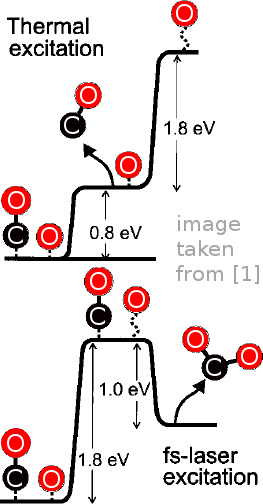
\includegraphics[width=.65\textwidth]{figures/CO_CO2.png}
      \end{figure}\vspace{-.5cm}                  
    \begin{center}  		
	\begin{footnotesize}CO/O-coadsorbate @ Ru(0001)\end{footnotesize} \\ \begin{scriptsize}M. Bonn \textit{et al.}, \textit{Science} 1999 \end{scriptsize}
    \end{center}
      
%     \end{block}
%   \end{columns}  
\end{frame}

% \begin{frame}{CO/Ru-System}


\begin{frame}{Specific motivation for investigating CO/Ru(0001)}
  \begin{block}{CO/Ru(0001) system important for catalysis, e.g.:}
	\begin{itemize}
	  \item Fischer-Tropsch synthesis {($n\,$CO + 2$n\,$H$_2 \rightarrow$ Alkane/Alkene/Alkohole + H$_2$O)} 
	  \item exhaust gas converters \begin{footnotesize} (cars, power plants, etc.)	                                               \end{footnotesize}
	\end{itemize}

  \end{block}
 
  \begin{block}{Experimentally well studied system}
    \begin{itemize}
	  \item especially regarding fs-laser irradiation:\begin{itemize}\item \begin{scriptsize}e.g. Bonn \textit{et al.}, \textit{Science} 1999; Funk \textit{et al.}, \textit{JChemPhys} 2000\end{scriptsize}	                                                                                                                                                      \item\begin{footnotesize}(both Ertl group $\Rightarrow$ chemistry Nobel prize 2007).	                                                                                                                                                                                                                                                                                                                                        \end{footnotesize}\end{itemize}
	  \item desorption kinetics: large prefactors $\Rightarrow$ still not understood 
	  \item recently, time resolved x-ray spectra (XAS and XES)
	  \newline $\Rightarrow$ ``movie'' of changes in orbital density of states
	  \begin{itemize}
	    \item {\scriptsize Dell'Angela \textit{et al.}, \textit{Science} 2013}
	  \end{itemize}

	  
%      \item Ultrafast time-resolved X-Ray-spectroscopy hints to physisorbed precursor state
%      \item Recent full 6D PES does not feature physisorption well
    \end{itemize}
  \end{block}
  
%   \begin{block}{Open questions for theory}
%     \begin{itemize}
%      \item Do dynamics reproduce other observables correctly? (e. g. desorption yield) 
%      \item Can the X-Ray-spectra also be explained without physisorption?
%     \end{itemize}
%   \end{block}
\end{frame}

\begin{frame}{Further specific motivation for investigating CO/Ru}{F\"uchsel \textit{et al.}, \textit{JChemPhys} 2014} 
  \vspace*{-.4cm}
  \begin{columns}
	\column{.5\textwidth}
	  \begin{figure}
		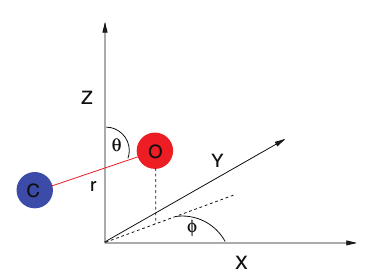
\includegraphics[width=.8\textwidth]{figures/6dimScheme.png}
	  \end{figure}
	\column{.5\textwidth}
	  \begin{figure}
		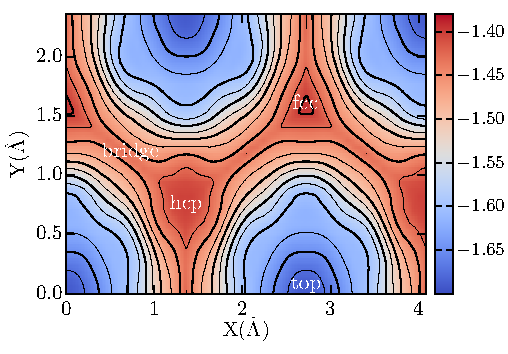
\includegraphics[width=.8\textwidth]{figures/PES_XYview.pdf}
	  \end{figure}
	
  \end{columns}
  \begin{block}{Important prior theory work was done at our group \newline{\scriptsize F\"uchsel \textit{et al.}, \textit{JChemPhys} 2014}}
  \begin{itemize} 
    \item Development of a potential energy surface (PES)
	  \begin{itemize}
	    \item \footnotesize from over 90$\,$000 DFT points!
	        \item all 6 dimensions of the adsorbate
    \item very fast because preconstucted\\~
    \item[\LARGE$\Rightarrow$] {\large\textbf{enables large-scale dynamics!}}
    	  \end{itemize}
  \end{itemize}
  \end{block}
\end{frame}


\subsection[101 of fs-lasers]{First impressions of fs-laser-driven dynamics}



\begin{frame}{What happens after fs-laser excitation of the metal?}
%   \begin{figure}
	\hspace*{-.5cm}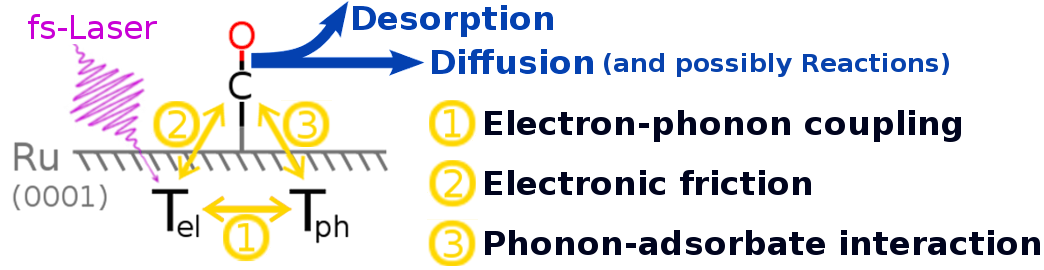
\includegraphics[width=1.1\textwidth]{figures/modifiedSurfScheme.png} 
%   \end{figure}

  \begin{columns}
  \column{0.8\textwidth}
  \begin{block}{Coupling between 3 kinds of degrees of freedom:} 
    \begin{itemize}                                                                   
      \item electron gas ($T_\mathrm{el}$) 
	\begin{itemize}
	  \footnotesize
	 \item initially absorbs laser energy
	 \item low heat capacity $\Rightarrow$ high $T_\mathrm{el}$ ($\approx$5-10$\,$kK)
	\end{itemize}
      \item lattice vibrations ($T_\mathrm{ph}$)
			\begin{itemize}
	  \footnotesize
	 \item thermalization with electrons: ps time scale
	 \newline $\Rightarrow$ fs-laser causes two distinct temperatures!
	\end{itemize}
      \item adsorbate movement ($T_\mathrm{ads}$)
    \end{itemize}

  \end{block}
  \column{0.2\textwidth}
  \begin{figure}
    \hspace*{-.2cm}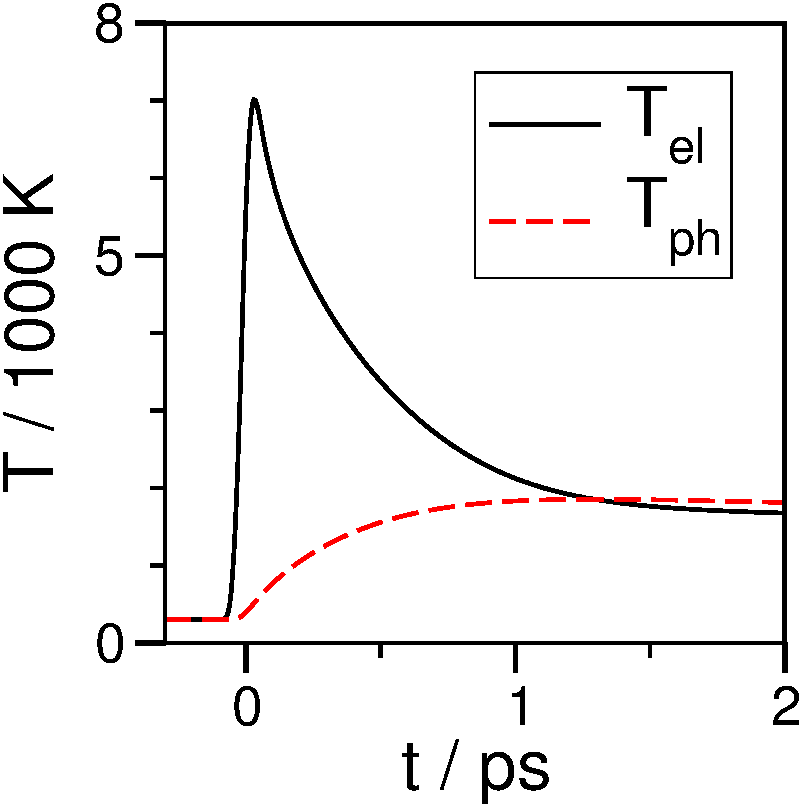
\includegraphics[width=1.3\textwidth]{figures/TTM_1pulse-eps-converted-to.pdf}
  \end{figure}
  \end{columns}
\end{frame}

\begin{frame}{Details of the time-resolved x-ray experiment}{Dell'Angela \textit{et al.}, \textit{Science} 2013 {\scriptsize (experimental part by Nilsson group, SLAC/LCLS, Stanford)}}
  \vspace*{-.7cm}
  \begin{columns}[t]
    \column{0.51\textwidth}
      \begin{block}{What was done?}
        \begin{itemize}
         \item pump: \textit{vis}-fs-laser 
         \item probe: x-ray free $e^{-}$ laser
		  \begin{itemize}\footnotesize
		    \item K-edge of O-atom
		  \end{itemize} 
        \end{itemize}

      \end{block}
%       \begin{block}{How does it work?}
%        
%       \end{block}	  
      \begin{block}{What is observed?}
        \begin{itemize}
	  \item orbital density of states at O 
	  \item energies shift towards gas-phase values of CO
	  \item intensities change 
	  \begin{itemize}
		\footnotesize
	   \item 2$\tilde{\pi}^*$ $\Rightarrow$ increase by $\sim30$\% 
	   \item \~{d}$_\pi$ $\,\Rightarrow$ decrease by $\sim30$\%
	   \item participator peak appears
	  \end{itemize}
	  \large \item[\LARGE$\Rightarrow$] physisorbed precursor(?)
	\end{itemize}	  
      \end{block}      
    \column{0.50\textwidth}
     \vspace*{-.8cm}
  \begin{figure}
    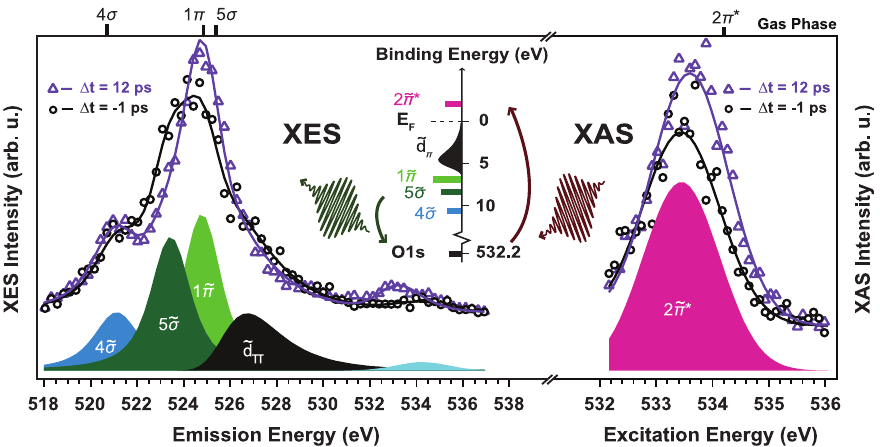
\includegraphics[width=1.1\textwidth]{figures/scienceXray.png}
  \end{figure}
         \vspace*{-.15cm}
%   \begin{figure}
    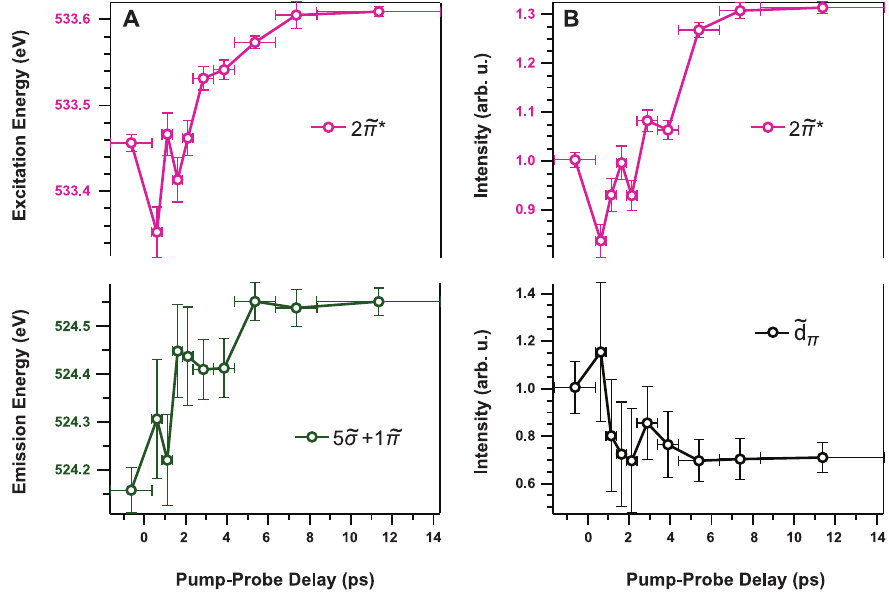
\includegraphics[width=1.1\textwidth]{figures/XrayIntOverTime.png}
%   \end{6figure}
  \end{columns}
\end{frame}

\begin{frame}{Details of the accompanying theory}{still Dell'Angela \textit{et al.}, \textit{Science} 2013 {\scriptsize (theory part by N\o{}rskov group, SUNCAT, Stanford)}}
  	\vspace{-1cm}
  \begin{columns}[t]
  \column{0.55\textwidth}
	\vspace{-.53cm}
	\begin{figure}
	  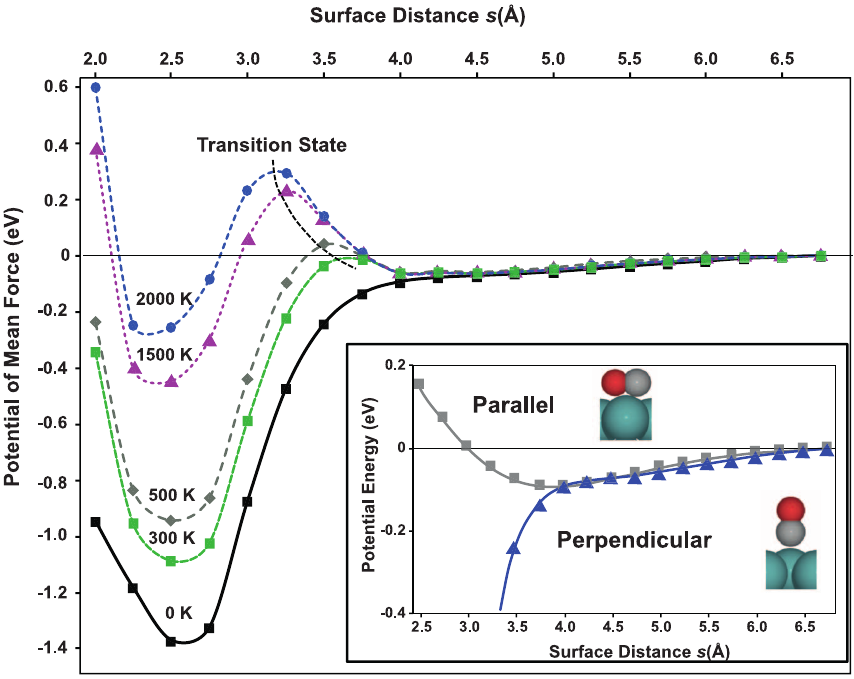
\includegraphics[width=1.06\textwidth]{figures/sciencePMF.png}
	\end{figure}
	\vspace{.21cm}
	{\scriptsize \begin{center}
Dell'Angela \textit{et al.}, \textit{Science} 2013	                                                               \end{center}}
  \column{0.45\textwidth}
	\begin{figure}
	  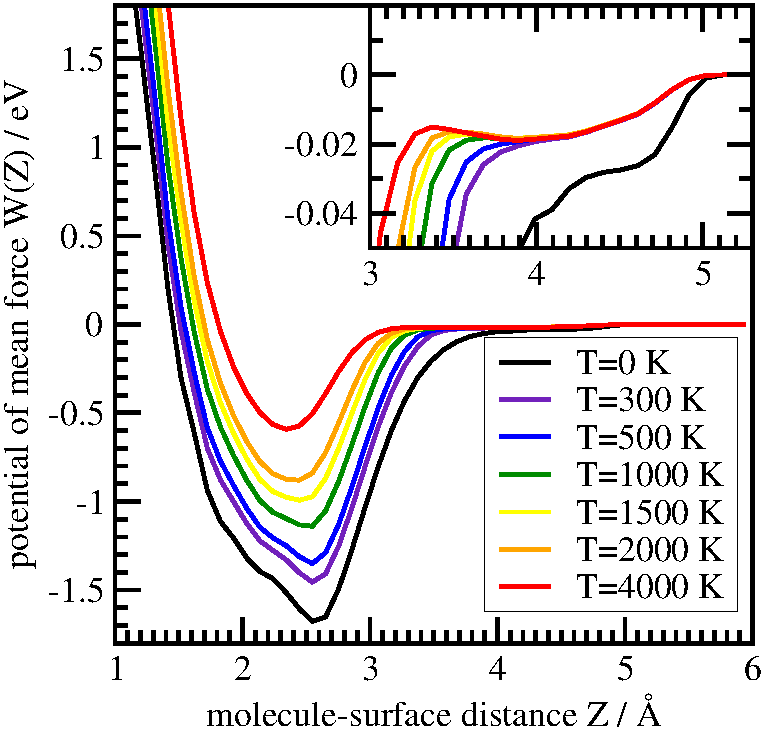
\includegraphics[width=1.1\textwidth]{figures/GernotPMF.pdf}
	\end{figure}
	{\scriptsize \begin{center}
Scholz \textit{et al.}, \textit{PhysRevB} 2016	                                                           \end{center}}
  \end{columns}


\end{frame}



\section{Models and methods}

% \subsection{The foundation: our 6D potential energy surface (PES)}
\subsection[6D PES and TTM]{Foundations: 6D potential and two-temperature model}
\begin{frame}{More facts about the potential energy surface (PES)}
  \begin{columns}
   \column{0.9\textwidth}
     
  \begin{block}{How was it constructed?}
    \begin{itemize}
      \item GGA-level (RPBE) with VdW-correction (D2)

      \item (2x2) cell with 1 CO $\Rightarrow$ 14 atoms, 0.25 ML coverage
      \begin{itemize}
	\item \footnotesize all 6 dimensions of adsorbate $\Rightarrow$ surface atoms frozen
      \end{itemize} 
      \item interpolation with cubic splines and\newline corrugation reducing procedure (CRP)
      \begin{itemize}
	\item \footnotesize atomic potentials temporarily substracted \newline $\Rightarrow$ smoother intermittent potential, interpolates better
      \end{itemize}
      \item slightly newer PES: C$_{3v}$- instead of C$_{6v}$-symmetry	
      \begin{itemize}
	\item \footnotesize differences between hcp and fcc sites not neglected
      \end{itemize}
     \end{itemize}

  \end{block}

   \column{0.15\textwidth}
       \begin{figure}
	\hspace*{-.2cm}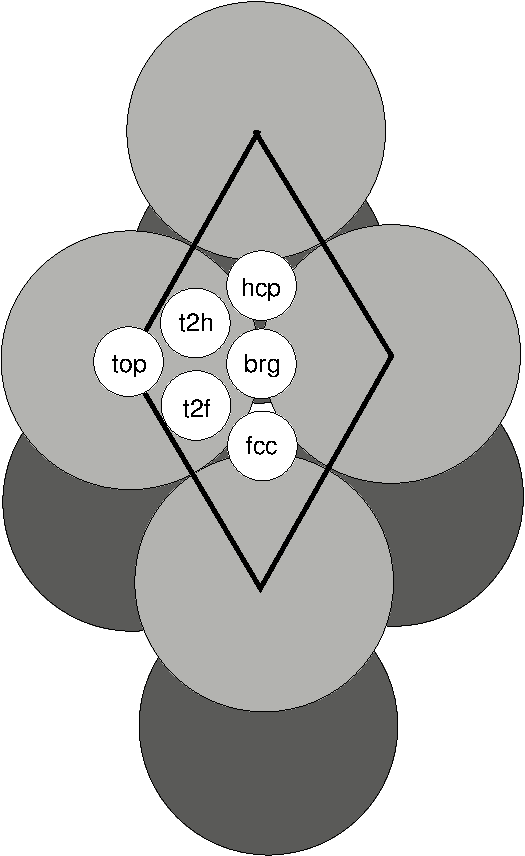
\includegraphics[width=1.3\textwidth]{figures/PES_samplepoints.pdf}
      \end{figure}
      
%       \begin{figure}
% 	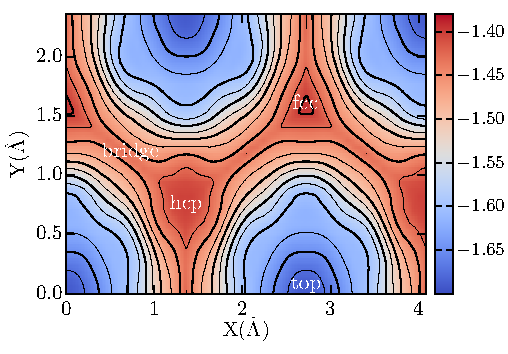
\includegraphics[width=1.2\textwidth]{figures/PES_XYview.pdf}
%       \end{figure}

  \end{columns}
        \begin{figure}
	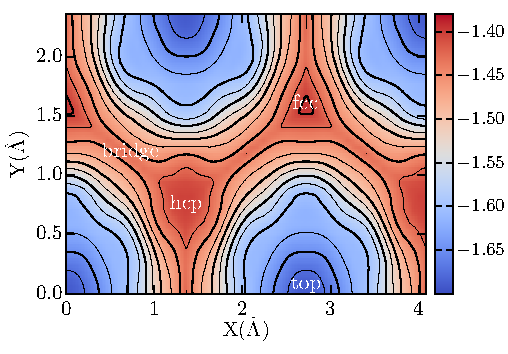
\includegraphics[width=0.33\textwidth]{figures/PES_XYview.pdf}
      \end{figure}
\end{frame}

% \subsection{The two-temperature model (TTM)}
\begin{frame}{Two-temperature model (TTM)}
  \begin{figure}
	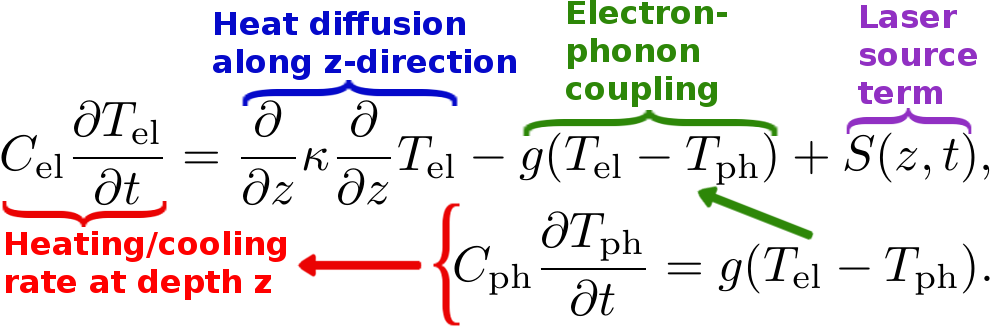
\includegraphics[width=\textwidth]{figures/2TM_equs.png}
  \end{figure}
  \begin{figure}
    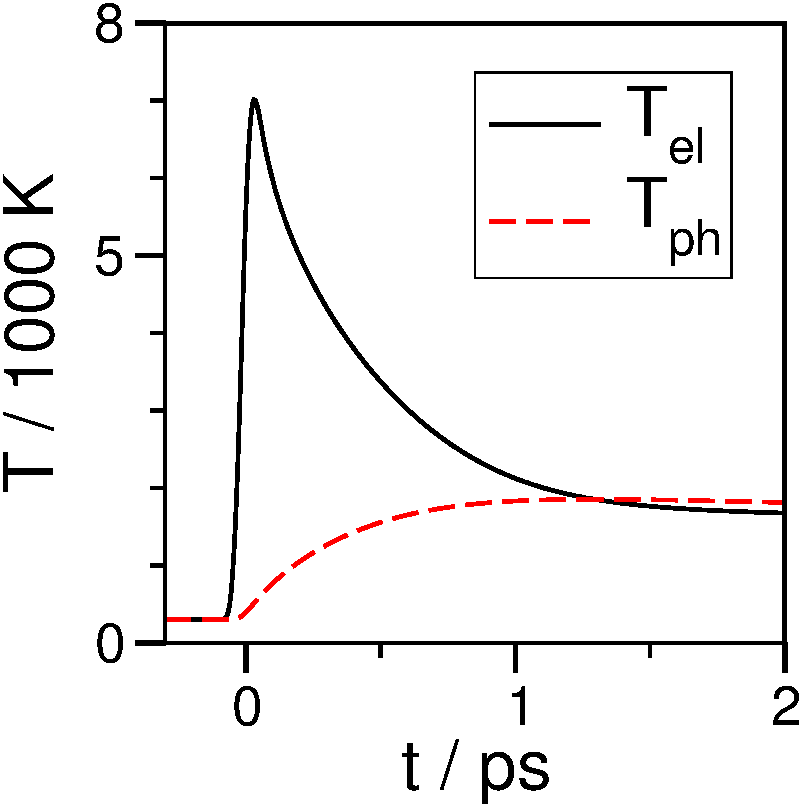
\includegraphics[width=.35\textwidth]{figures/TTM_1pulse-eps-converted-to.pdf}
  \end{figure}  
\end{frame}


\subsection[MDEF]{Electronic friction: non-adiabatic coupling approximated}
\begin{frame}{Different approaches to non-adiabatic coupling}
  \begin{figure}
	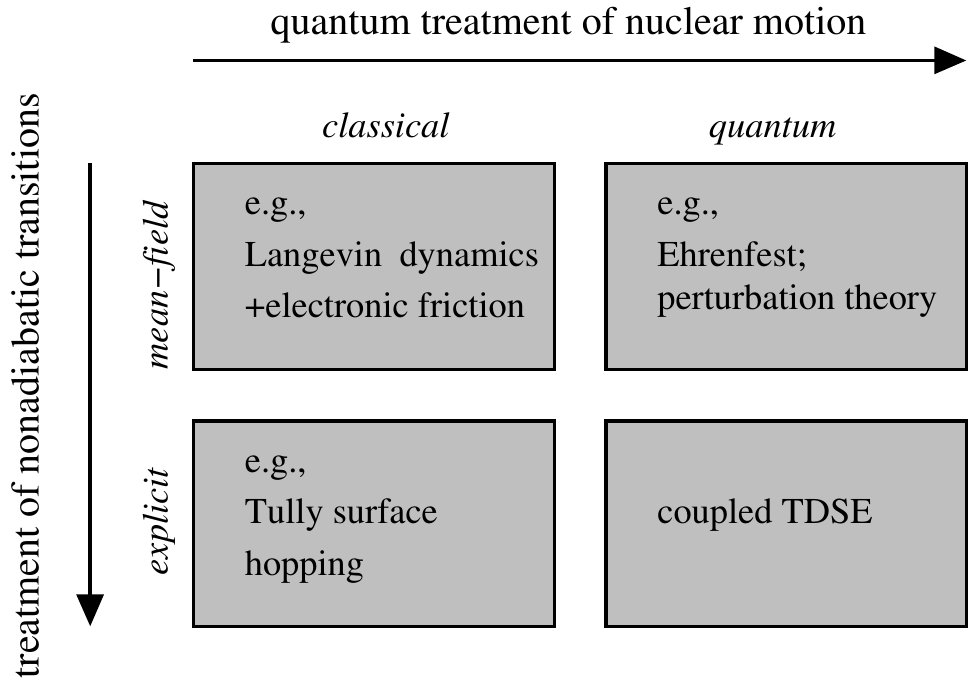
\includegraphics[width=.6\textwidth]{figures/scheme_nonadiab.png}
  \end{figure}
  \begin{block}{Langevin dynamics + electronic friction}
   \begin{itemize}
    \item fastest method $\Rightarrow$ suited for multi-dimensional dynamics
    \item good approximation for weak non-adiabatic coupling
   \end{itemize}

  \end{block}

\end{frame}

\begin{frame}{The Langevin equation}{A stochastic differential equation}
  \begin{columns}
  \column{0.3\textwidth}
   \begin{figure}
	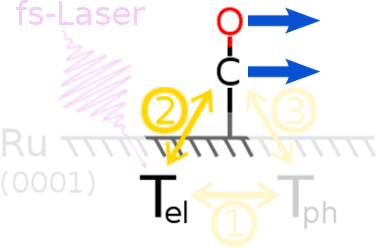
\includegraphics[width=\textwidth]{figures/Part2SurfScheme.png}
  \end{figure}
  \column{0.8\textwidth}
\begin{figure}
	
\includegraphics[width=\textwidth]{figures/Langevin_eq.png}
  \end{figure}
    \end{columns}
  \begin{block}{Langevin equation within IAA {\small(independent atom approx.)}}
  \begin{itemize}
   \item friction coefficient of Atom k: $\eta_{\mathrm{el},k}(\underline{r}_k)$ $\Rightarrow$ dissipation
  
      \begin{itemize}
      \footnotesize
      \item derived from local density friction approximation (LDFA)
      \newline $\Rightarrow$ individual atom (again IAA) in free electron gas
      \item $\eta_{\mathrm{el},k}(\underline{r}_k)$ dependent on electron density of bare surface
      \end{itemize}

    \item random force $\underline{R}_{\mathrm{el},k}(t)$ $\Rightarrow$ fluctuation% 
%     \item 
     
    \begin{itemize}\footnotesize
	  \item Gaussian white noise
	  \item describes excitation by hot electron-hole pairs
      \item proportional to: $\eta_{\mathrm{el},k}(\underline{r}_k)$ and $T_\mathrm{el}(t)$
    \end{itemize}
  \end{itemize}
  \end{block}
\end{frame}

% \begin{frame}{Local density friction approx. plus independent atoms} 
%   
% \end{frame}

\subsection[GLO]{The generalized Langevin oscillator (GLO)}
\begin{frame}[plain]{Generalized Langevin Oscillator}
  \begin{columns}[c]
    \column{0.25\textwidth}
	  \vspace{-1.9cm}
	  \begin{figure}
		\hspace*{-.7cm}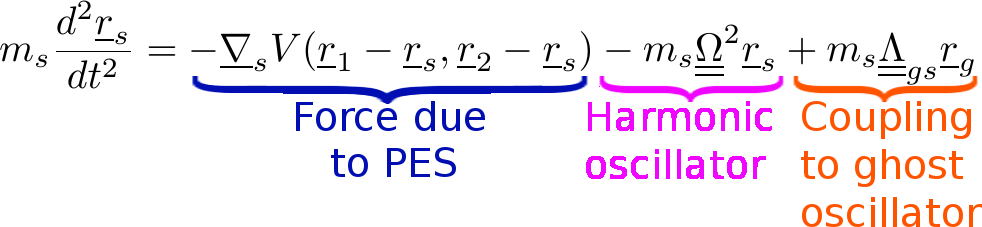
\includegraphics[width=2.6\textwidth]{figures/GLO_eq1.png}
	  \end{figure}
	  \vspace{2.7cm}
	  \begin{figure}
		\hspace*{-.7cm}
\includegraphics[width=2.4\textwidth]{figures/GLO_eq2.png}
	  \end{figure}
	\column{.68\textwidth}
% 	  \begin{figure}
		\hspace*{-.7cm}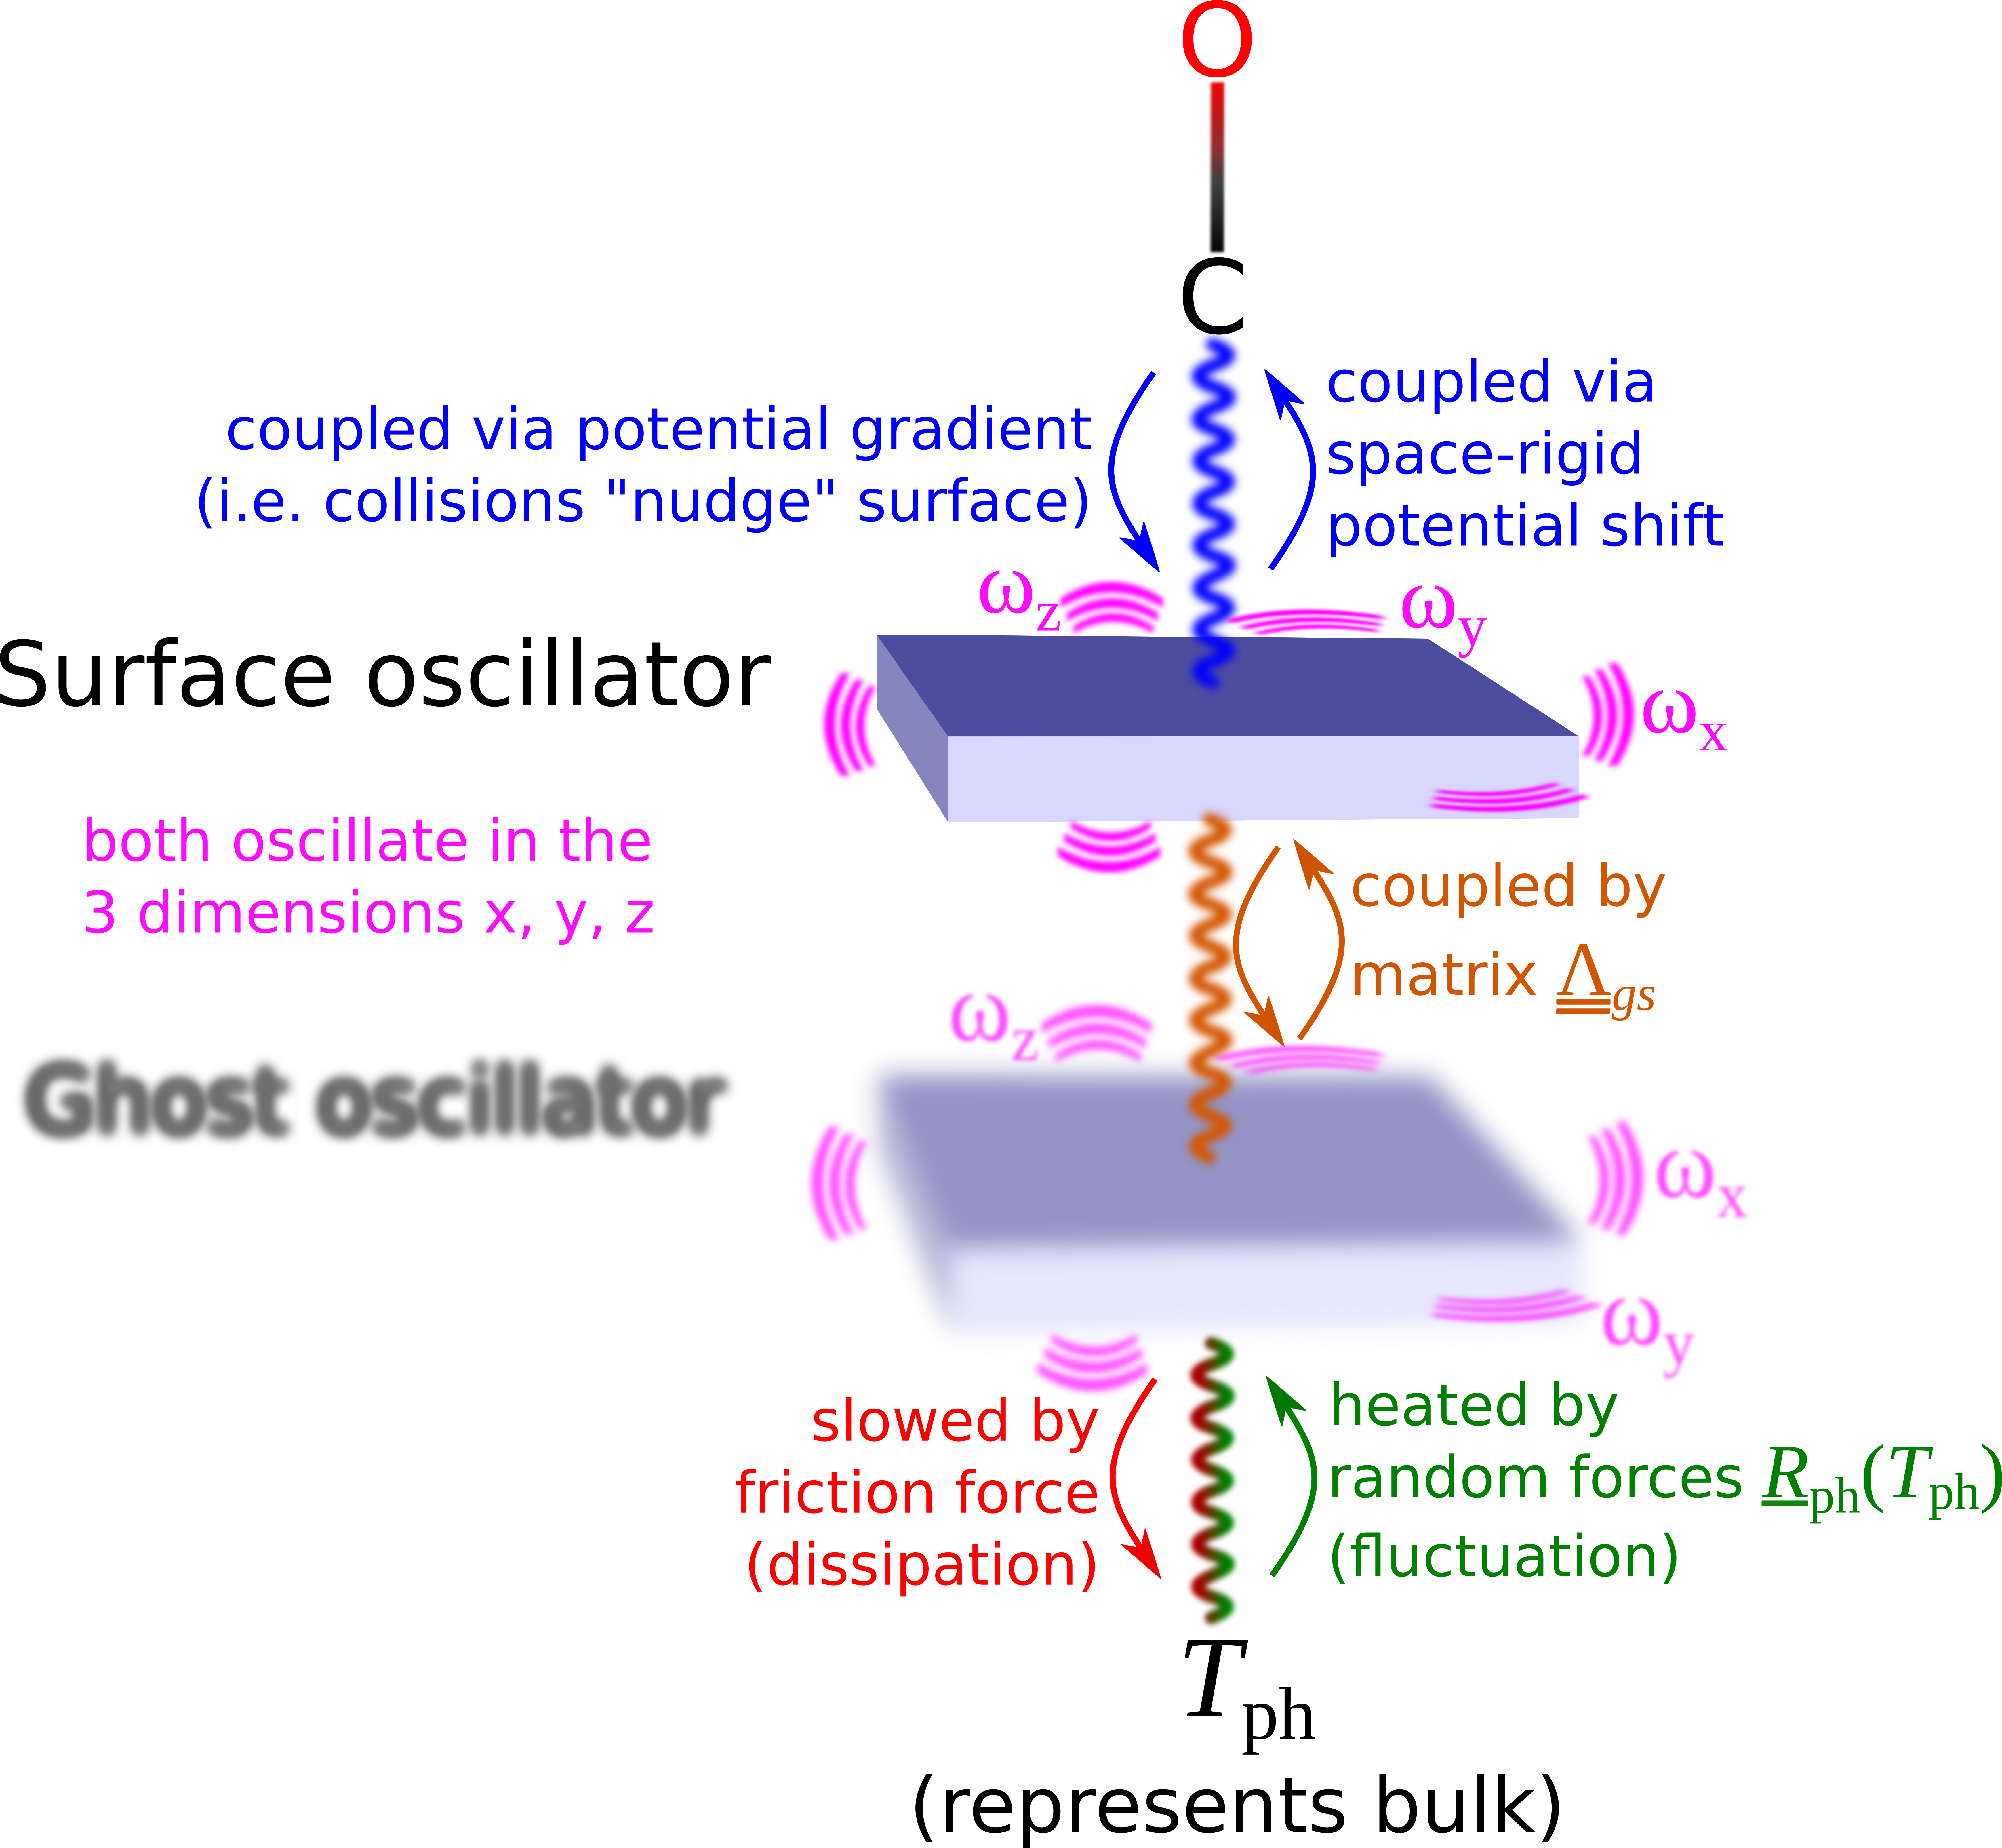
\includegraphics[width=1.2\textwidth]{figures/GLO.png}
% 	  \end{figure}
  \end{columns}
\end{frame}

\subsection[Half-time]{``Half-time'': short summary {\scriptsize(and maybe time for a few questions)}}

\begin{frame}{Summary of models and methods}
  \begin{figure}
	\hspace*{-.85cm}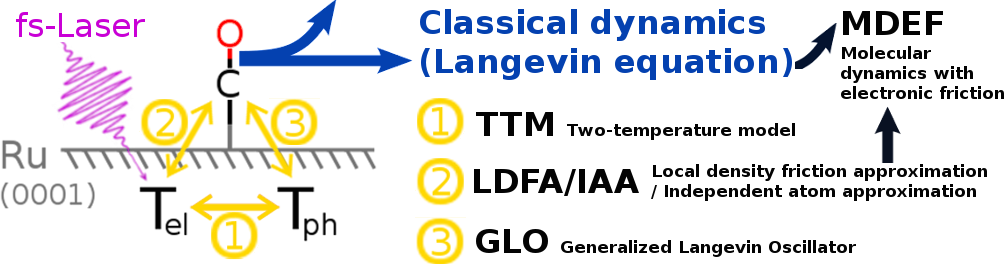
\includegraphics[width=1.15\textwidth]{figures/SummSurfScheme.png}
  \end{figure}
\end{frame}


\section{Results and discussion}

\subsection{Overview of computational settings}

\begin{frame}{Overview of computational settings}
  \begin{figure}
% 	\includegraphics[width=\textwidth]{figures/}
  \end{figure}
\end{frame}

\subsection{Laser-driven diffusion and desorption}

\begin{frame}{Example trajectory}{(in this case without GLO-model)}
  \begin{figure}
	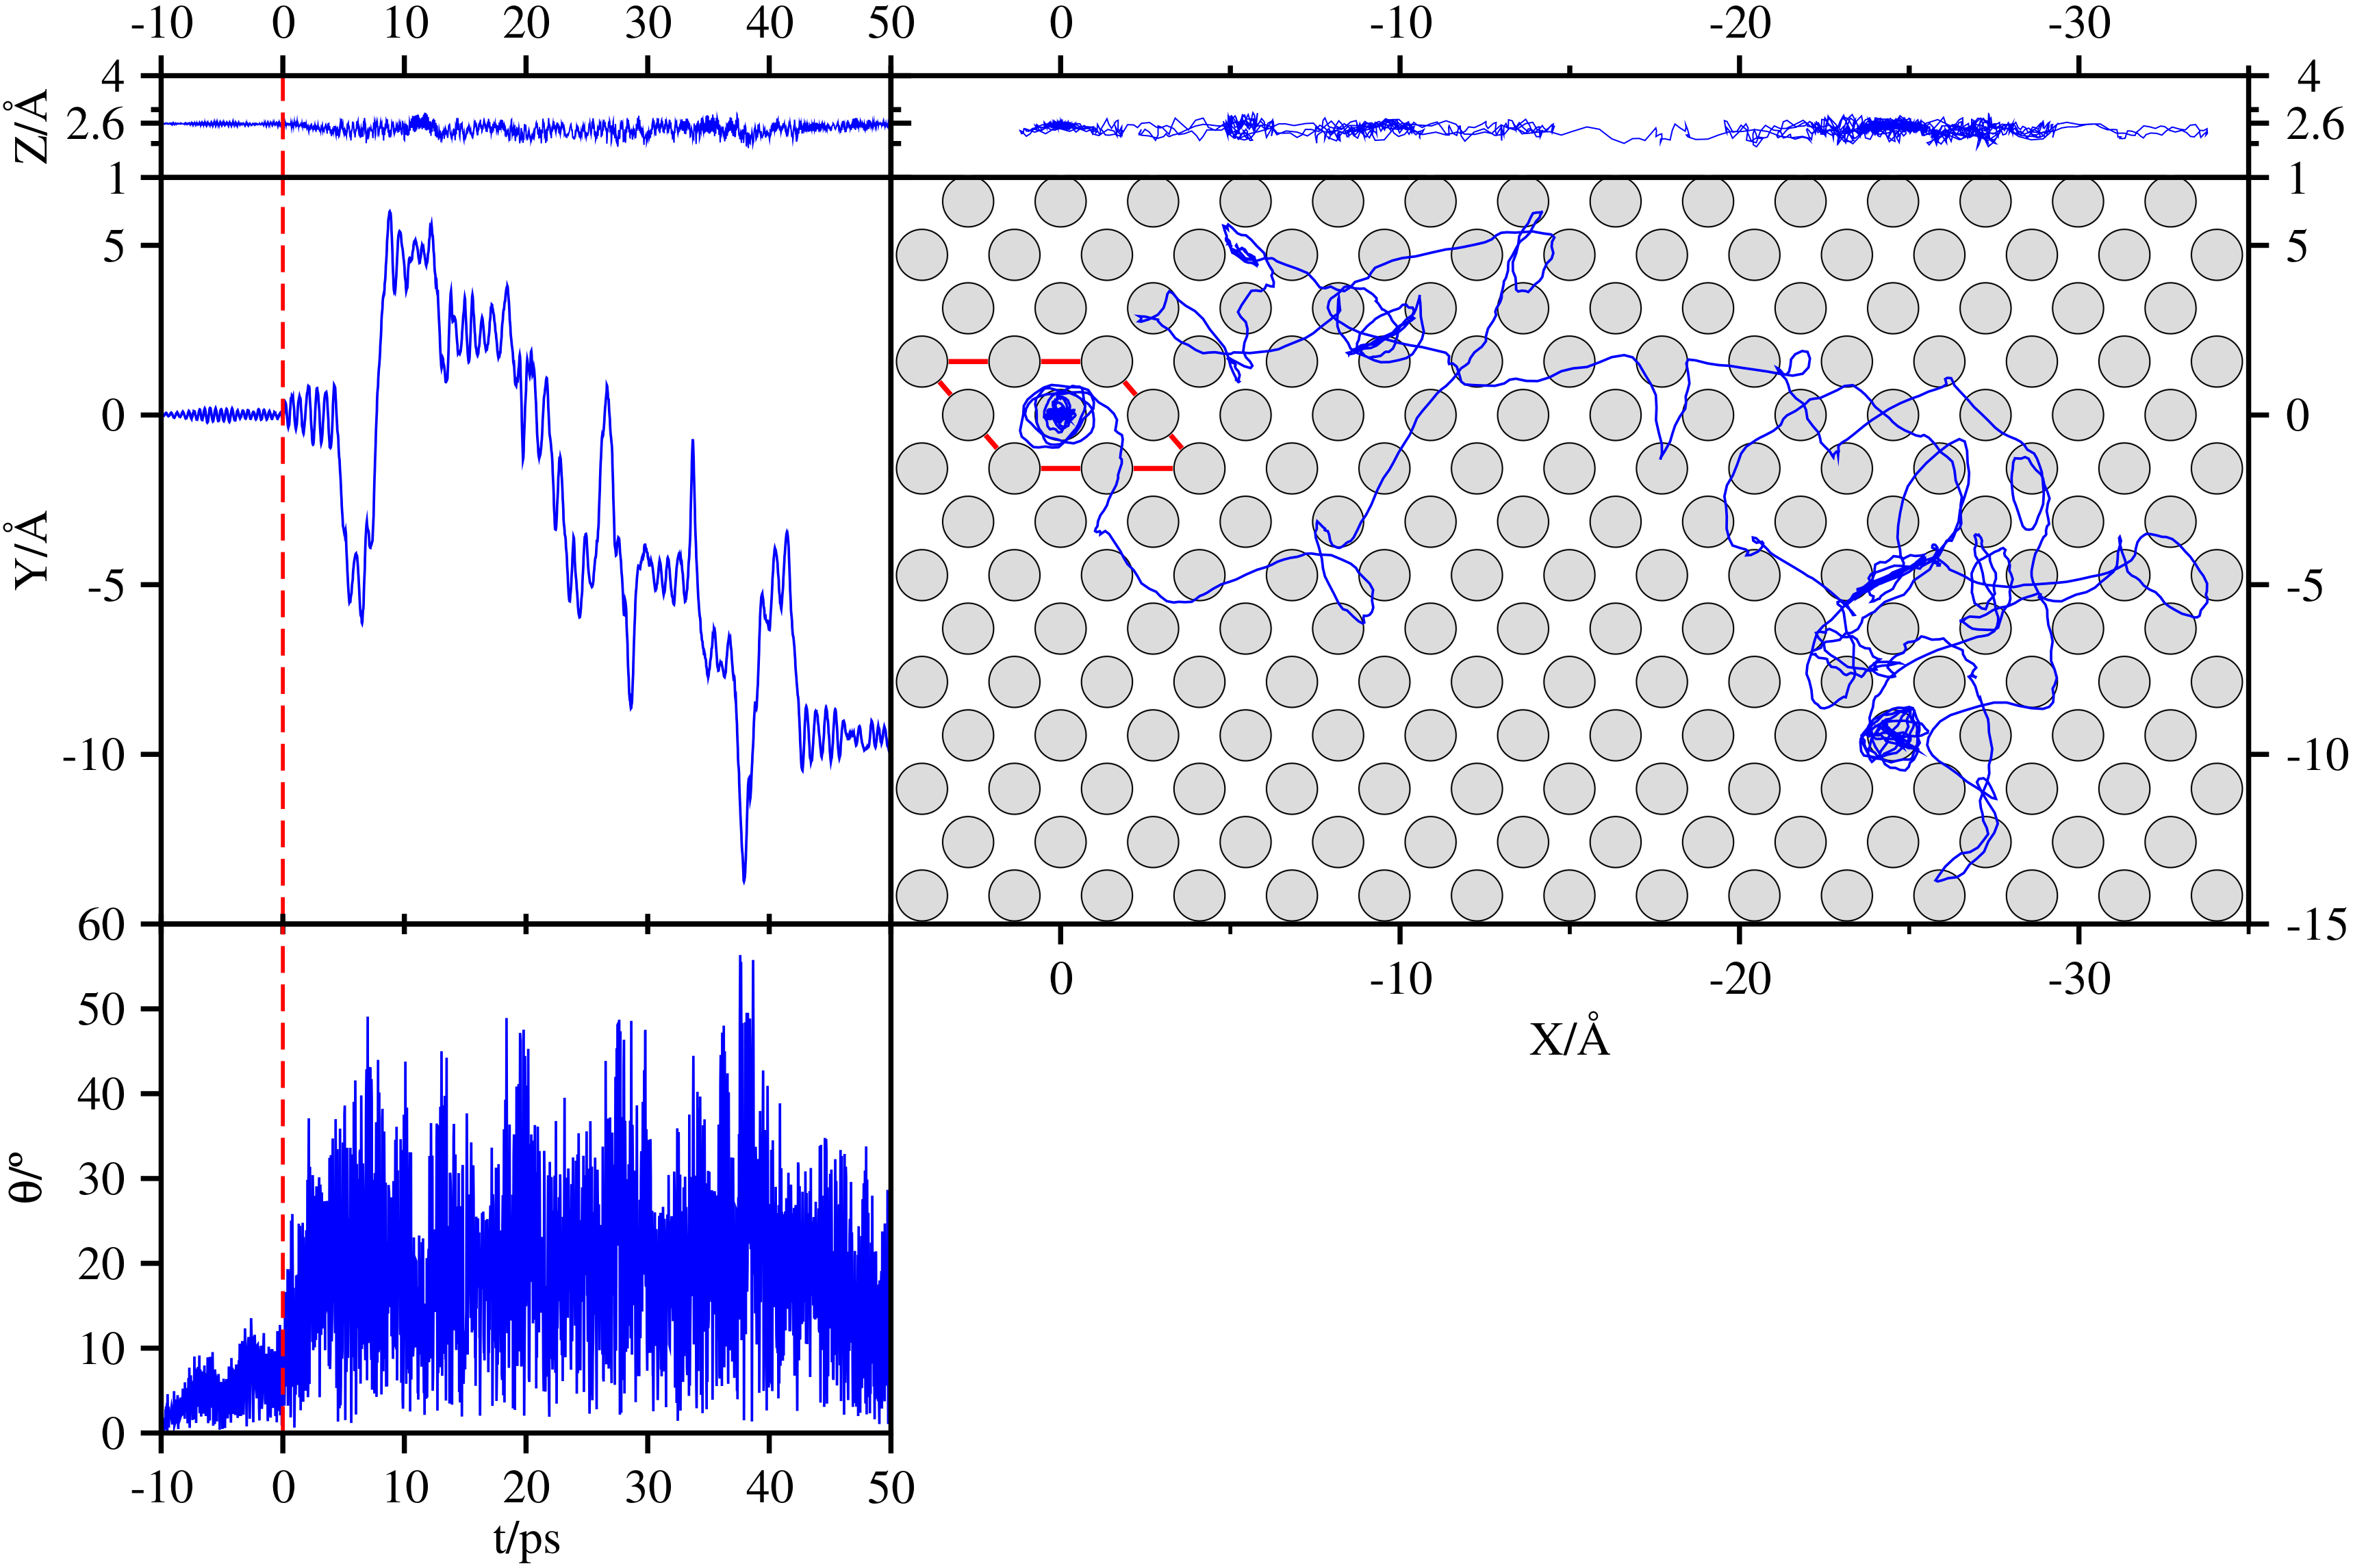
\includegraphics[width=\textwidth]{figures/Traj_XYZTh.png}
  \end{figure}
\end{frame}

\begin{frame}{Heating of DOFs $Z$ and $\theta$}
  \begin{figure}
	\vspace*{-.4cm}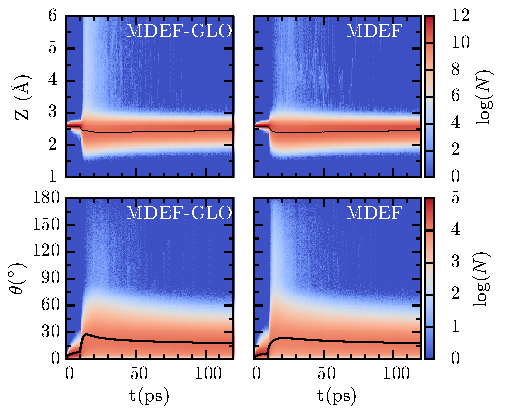
\includegraphics[width=.9\textwidth]{figures/ZundTheta.pdf}
  \end{figure}
\end{frame}

\begin{frame}{Fluence-dependence of desorption yield $P_\mathrm{des}$}
  \begin{columns}
    \column{.75\textwidth}
    \begin{figure}
      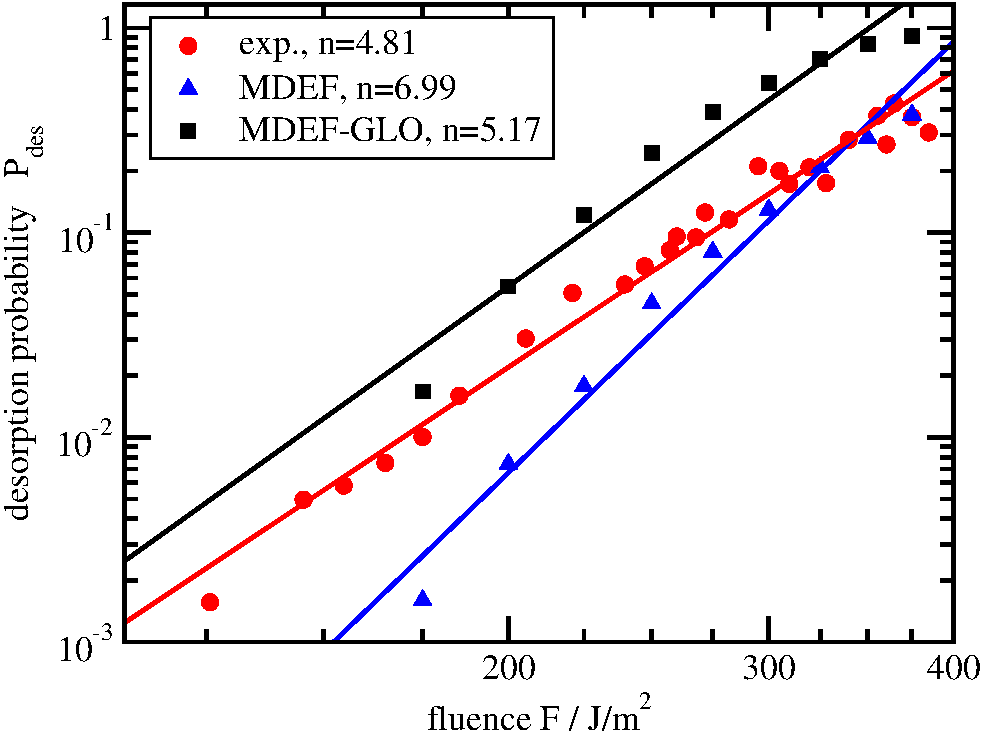
\includegraphics[width=1\textwidth]{figures/Pdes_vs_Fluence.pdf}
    \end{figure}
    \column{.3\textwidth}
      \begin{block}{Power-law}
	\begin{itemize}
	 \item $P_\mathrm{des} = A \cdot F^n$
	 \item not exactly
	\end{itemize}

      \end{block}
      
      \begin{block}{Differences in exp.}
	\begin{itemize}
	 \item coverage:
	 \item  [$\Rightarrow$] \begin{small}0.68 ML (max.)	                                      \end{small}
	\end{itemize}

      \end{block}

  \end{columns}
\end{frame}

% \begin{frame}{Two-pulse correlation of desorption}
%   \begin{figure}
% 	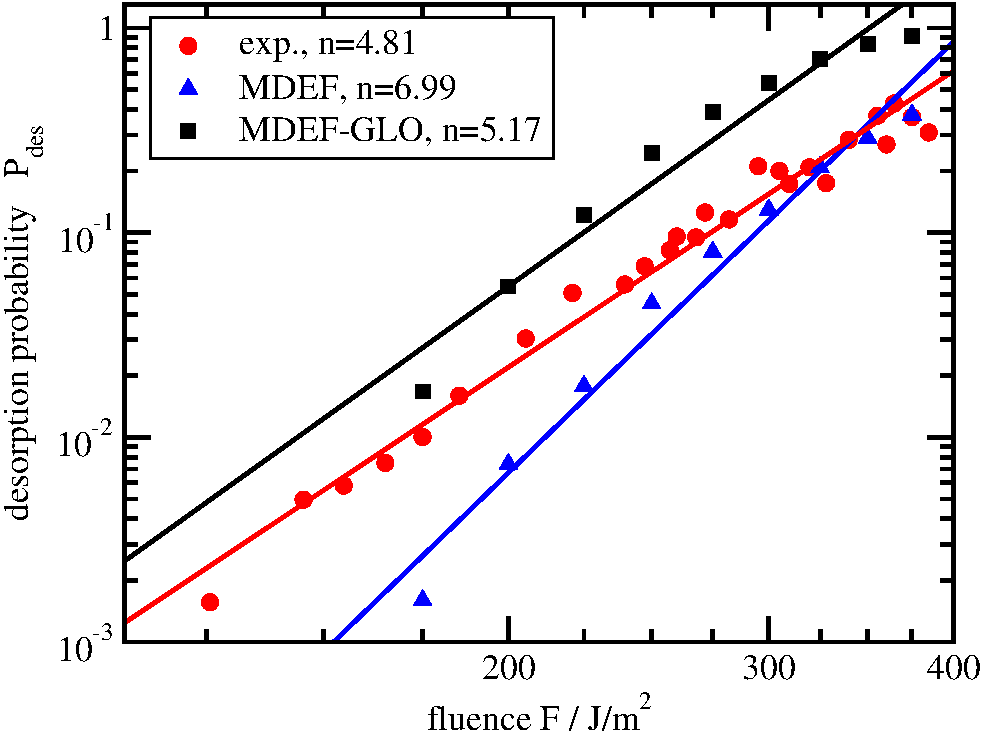
\includegraphics[width=.7\textwidth]{figures/Pdes_vs_Fluence.pdf}
%   \end{figure}
% \end{frame}

\subsection{Physisorbed precursor states?}

\begin{frame}{No population of physisorbed state in our dynamics}{As is to be expected from negligible barrier in potential of mean force (PMF)}
  \begin{columns}
  \column{0.6\textwidth}
    \begin{figure}
      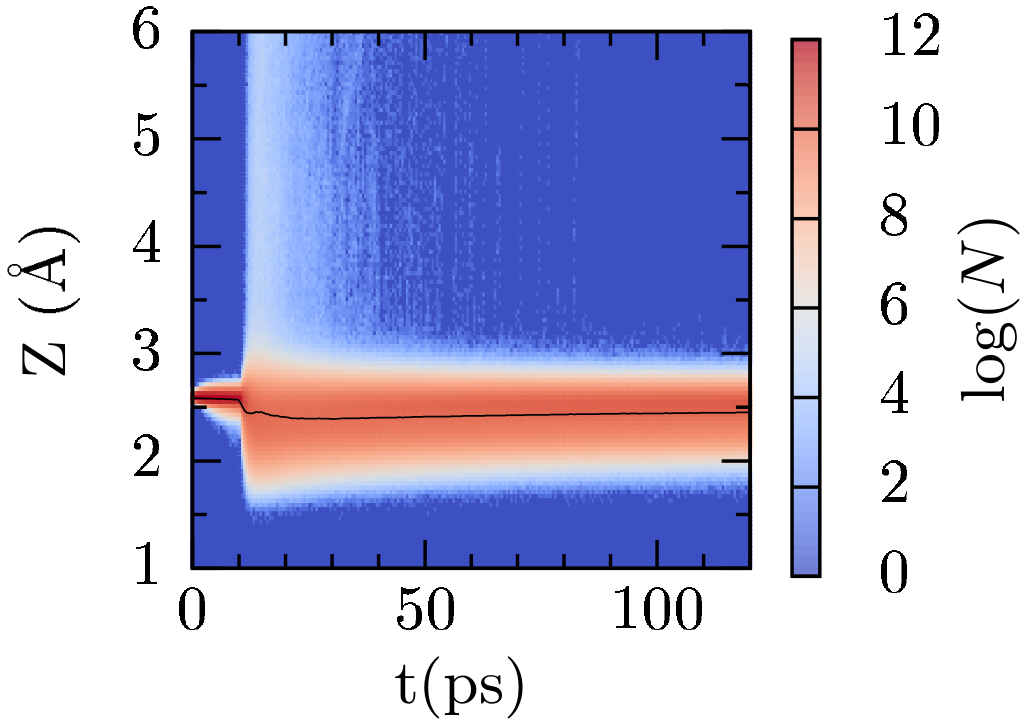
\includegraphics[width=1.\textwidth]{figures/NurZ.png}
    \end{figure}
  \column{0.4\textwidth}
    \begin{figure}
      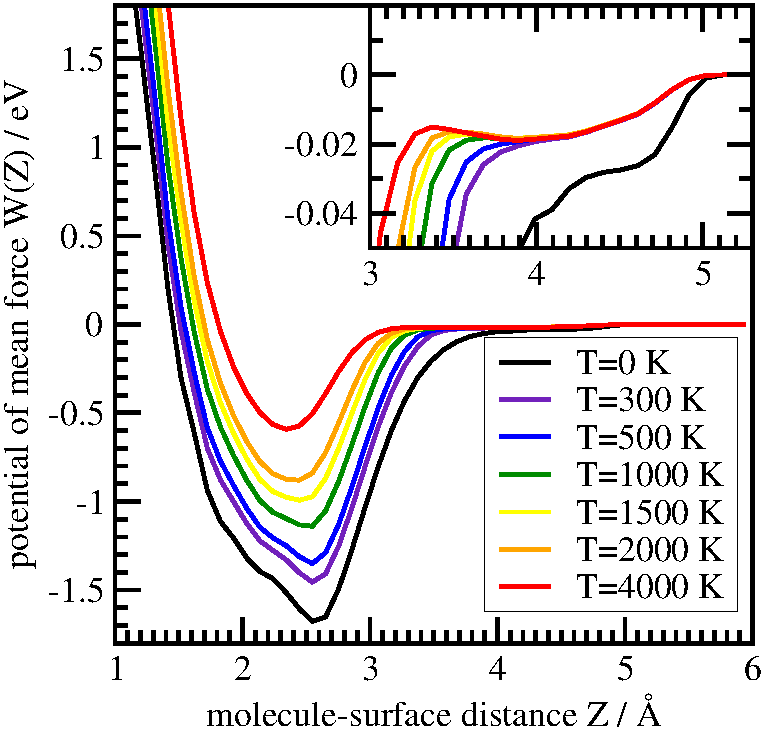
\includegraphics[width=1.\textwidth]{figures/GernotPMF.pdf}
    \end{figure}
  \end{columns}
\end{frame}

\begin{frame}{Why are the entropic barriers of the PMFs so different?}
  \begin{block}{Because separability assumption fails clearly}
    \begin{itemize}
     \item if introduced for our PMF $\Rightarrow$ barrier of similar heigth!
     \item expectable, because $X/Y$ and $\theta$ strongly coupled
    \end{itemize}
  \end{block}
  \begin{columns}
    \column{0.5\textwidth}
    \begin{figure}
      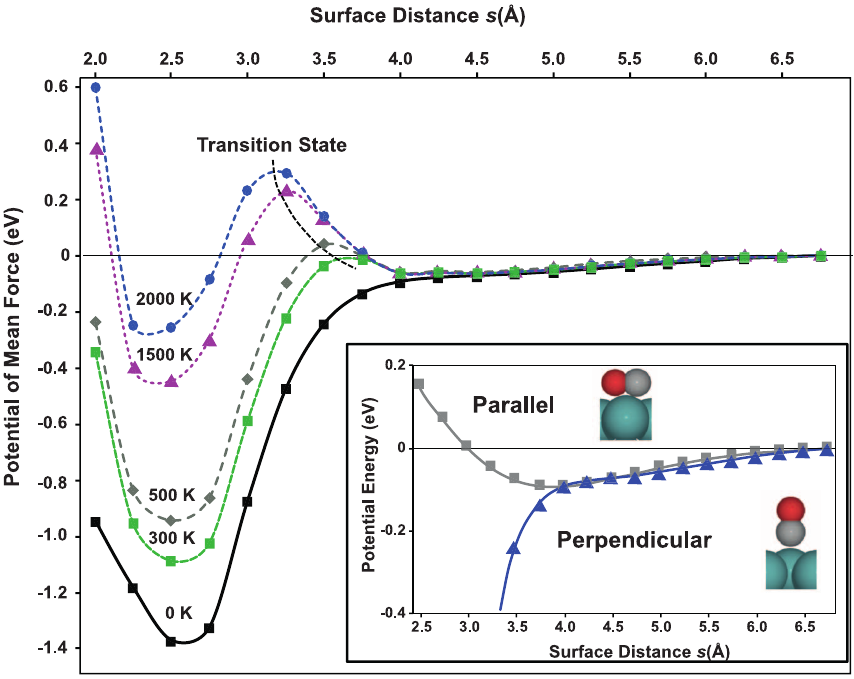
\includegraphics[width=\textwidth]{figures/sciencePMF.png}
    \end{figure}
    \column{0.5\textwidth}
    \begin{figure}
      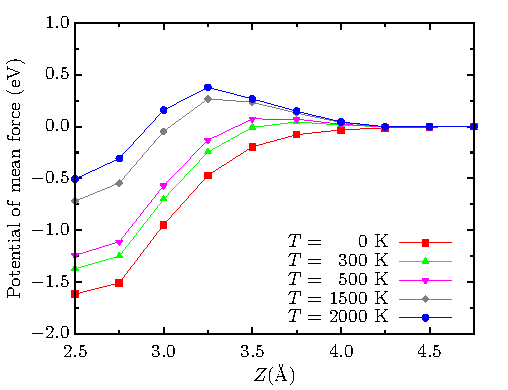
\includegraphics[width=\textwidth]{figures/PMF_Supp.pdf}
    \end{figure}   
  \end{columns}
\end{frame}



\begin{frame}{Dynamical trapping: {\normalsize alternative/additional explanation?}}

%     \begin{figure}
      \hspace*{-.6cm}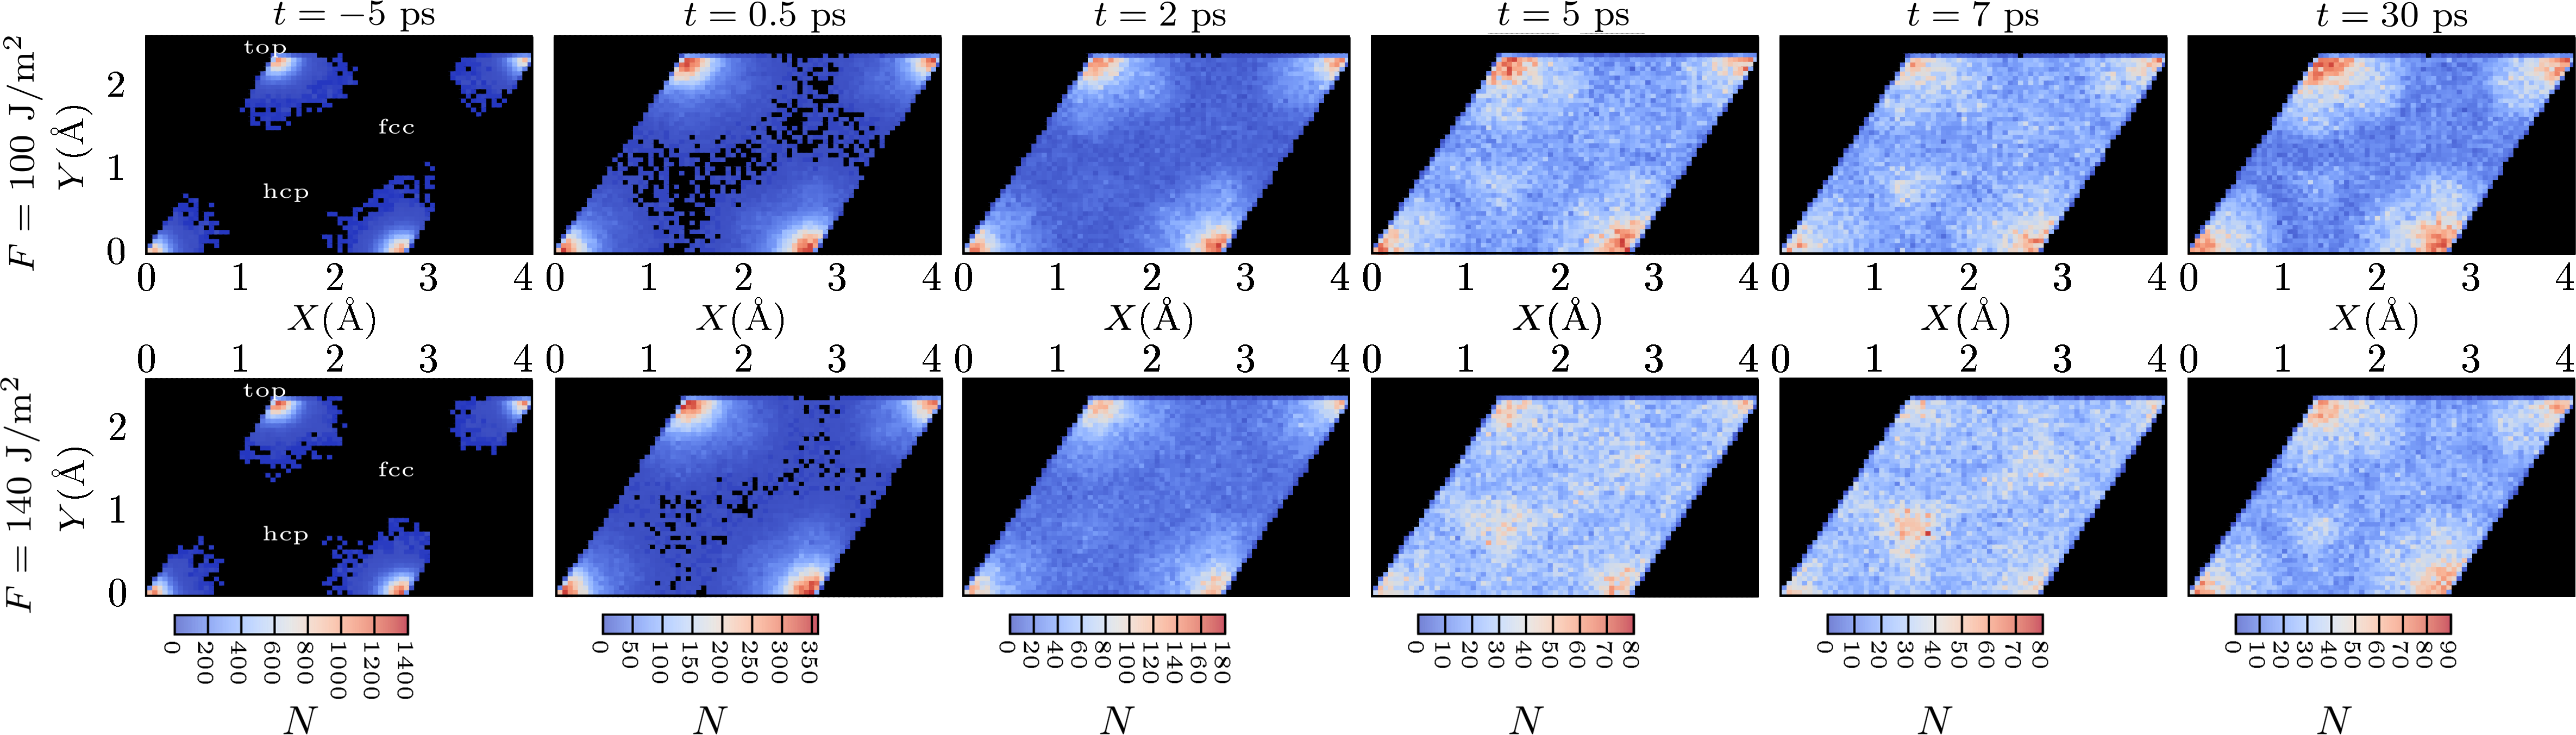
\includegraphics[width=1.1\textwidth]{figures/XYoverTime.png}
%     \end{figure}
\vspace*{-.5cm}
      \begin{columns}[t]
  \column{.65\textwidth}
  \begin{block}{Suprising patterns in XY-distribution}
    \begin{itemize}	  
      \item preferation of \textbf{hcp-site} after 5-7$\,$ps,
%       \item[$\Rightarrow$] 
      \newline despite it being a local maximum!
      \newline \textbf{$\Rightarrow$ dynamical trapping} {\footnotesize(cf. 30$\,$ps)}
      \item effect dependent on fluence
      \newline $\Rightarrow$ consistent with experiment \newline{\footnotesize(weaker ``precursor''-signal for lower fluence)}
    \end{itemize}   
  \end{block}

  \column{.4\textwidth}
    \begin{figure}
      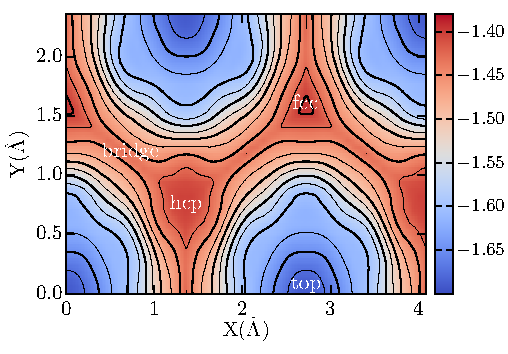
\includegraphics[width=\textwidth]{figures/PES_XYview.pdf}
    \end{figure}
  \end{columns}  
\end{frame}

\begin{frame}{Is there a physisorbed precursor state nevertheless?}
  \begin{columns}
    \column{0.7\textwidth}
    \begin{figure}
      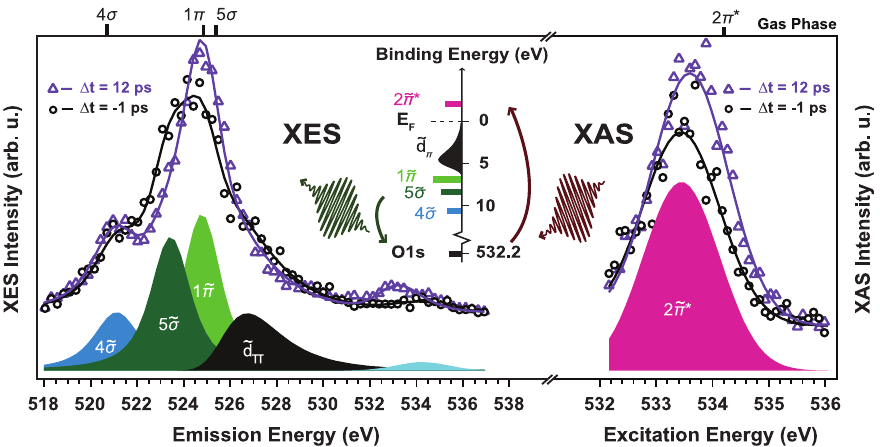
\includegraphics[width=1.\textwidth]{figures/scienceXray.png}
    \end{figure}      
    \column{0.2\textwidth}
    \begin{figure}
      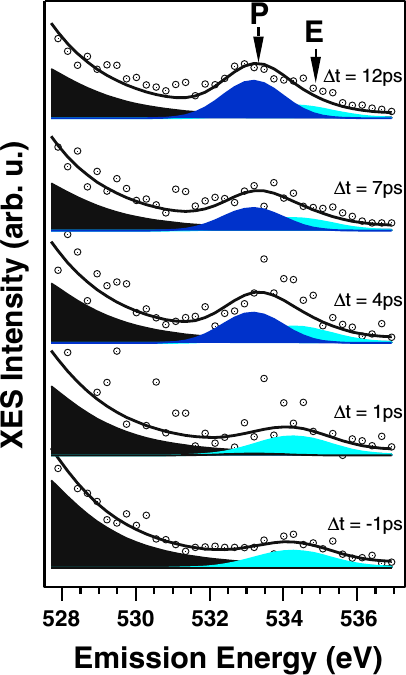
\includegraphics[width=1.\textwidth]{figures/PartiPeak.png}
    \end{figure} 
  \end{columns}
    \begin{block}{Dynamical trapping can't explain all observations}
      \begin{itemize}
        \item XAS of hcp-site computed: 2$\pi^*$-intensity not increased
	\item participator peak not explained by any XY-redistributions
	\newline $\Rightarrow$ Existence of physisorbed state very likely
	  \item but nevertheless not stable for Ru(2x2):CO models 
	 \newline $\Rightarrow$ probably stabilized by CO-CO-interactions 


	
      \end{itemize}
    \end{block}
\end{frame}


\section{Summary and Outlook}

  \begin{frame}[plain]{Outline}
    \tableofcontents[currentsection]
  \end{frame}

\begin{frame}{Summary}

\end{frame}

\begin{frame}{Outlook}

\end{frame}



% % \section{Einleitung}
% %   \subsection{Diamantoide - Die etwas anderen Nanodiamanten}
% \begin{frame}[plain]{Die Stoffklasse der Diamantoide}
%   \begin{block}{Was sind Diamantoide?}
%     \begin{itemize}
%      \item k\"afigartige, aliphatische Kohlenwasserstoffe
%      \item Kohlenstoffger\"ust wie im Diamantgitter 
%     \end{itemize}
%   \end{block}
%   \begin{columns}[t]
%    \column{.73\textwidth}
%     \begin{block}{Niedere Diamantoide}  
%       \begin{figure}
% 	\includegraphics[width=\textwidth]{../abb/low_diam_hres.png}
% 	\newline\begin{scriptsize}Abb. entnommen aus \alert{Fokin et al. 2008}	\end{scriptsize}
%       \end{figure}
%     \end{block}
% 
%    \column{.32 \textwidth}
%     \begin{block}{H\"ohere Diamantoide}
%       \begin{itemize}
%        \item Tetramantane \newline(4 Isomere)
%        \item Pentamantane \newline(10 Isomere)
%        \item und viele weitere
%       \end{itemize}  
%     \end{block}
%   \end{columns}
% \end{frame}


% \begin{frame}[plain]{Abgrenzung zu Nanodiamantmaterialien und Anwendungspotentiale}
%   \begin{columns}[t]
%   \column{.5\textwidth}
%   \begin{block}{Nanodiamanten}
%        \begin{itemize}
%      \item inhomogene Mischung vieler Verbindungen
%      \item Verklumpung $\Rightarrow$ relativ gro\ss{}e Partikel ($\approx100\,$nm)
%      \item hergestellt z. B. mittels
% 	  \begin{itemize}
% 	    \item Gasphasenabscheidung
% 	    \item Detonationssynthese
% 	  \end{itemize}
% 	\end{itemize}  
% 	\end{block}
%   \column{.5\textwidth}    
%   \begin{block}{Diamantoide}
% 	\begin{itemize}
%       \item isolierbare, chemisch reine Verbindungen
%       \item genau bekannte Struktur
%       \item Vorkommen: Erd\"ol, -gas, Sedimente      
%       \item kleinere Diamantoide auch synthetisierbar
% 	\end{itemize}
% 	\end{block}
%   \end{columns}
% 
% \begin{block}{Anwendungsm\"oglichkeiten f\"ur Diamantoide}
% 	\begin{itemize}
% 		\item Medizin
% 		\item Materialforschung, insbesondere Polymere
% 		\item Molekulare Elektronik
% 	\end{itemize}
% 
% \end{block}
% 
% \end{frame}
% 
% %   \subsection{Anwendungsbereiche von Diamantoidderivaten}
% 
% \begin{frame}[plain]{Eigenschaften und Anwendungsm\"oglichkeiten speziell f\"ur Adamantanthionderivate}
% \begin{columns}[t]
% \column{.7\textwidth}  
% \begin{block}{Adamantanthion}
% 	\begin{itemize}
% 		\item photochemisches Modellsystem f\"ur alicyclische Thioketone
% 	\end{itemize}
% 
% \end{block}
% \column{.3\textwidth} 
% \begin{figure}
% 		\includegraphics[width=\textwidth]{../abb/Thion.pdf}
% \end{figure}
% \end{columns}
% 
% \begin{columns}[c]
% 	\column{.5\textwidth}
%   \begin{block}{H\"oher substituierte Adamantanthionderivate}
%      \begin{itemize}
%       \item optische Bandl\"ucke im sichtbaren Bereich\footnote{\alert{V\"oros et al. 2012}}$^,$\footnote{\alert{St\"ucker 2013}}
%       \item m\"ogliche Verwendung als Biomarker$^a$
%      \end{itemize}
%   \end{block}
% \column{.5\textwidth}
% \begin{columns}[c]
% \column{.7\textwidth}
% \begin{figure}
% 		\includegraphics[width=1.15\textwidth]{../abb/optical_gap.png}
% \end{figure}
% \column{.3\textwidth}
% \begin{figure}
% 		\includegraphics[width=\textwidth]{../abb/ada.png}
% \end{figure}
% \end{columns}
% 		\begin{scriptsize}$\quad$Abb. entnommen aus Ref. a\end{scriptsize}
% \end{columns}
% \end{frame}
% %   \section{Theoretische Grundlagen}
%      
% \begin{frame}[plain]{Strahlende und strahlungslose \"Uberg\"ange}
% 
% \begin{columns}[c]
%  \column{.55\textwidth}
%   \begin{figure}
% 	\includegraphics[width=\textwidth]{../abb/Jablonski.png}
% 	\caption{Jablonski-Schema, entnommen aus \alert{Itoh 2012}}
%       \end{figure}
% 
%  \column{.5\textwidth}
%    \begin{block}{Strahlende \"Uberg\"ange}
%    \begin{itemize}
%     \item Absorption
%     \item Lumineszenz
%     \begin{itemize}
%      \item Fluoreszenz (F)
%      \item Phosphoreszenz (P)
%     \end{itemize}
%    \end{itemize}
% 
% 
%   \end{block}
%    \begin{block}{Strahlungslose \"Uberg\"ange}
%     \begin{itemize}
%      \item Internal Conversion (IC)\setbeamercolor{alerted text}{fg=red!80!black} 
%      \item<alert@1> Intersystem Crossing (ISC)
%      \item Vibrational Cooling (Vib) 
%     \end{itemize}
%   \end{block} 
%   \end{columns}
% \end{frame}
% \setbeamercolor{alerted text}{fg=green!40!black}
% 
% \begin{frame}[plain]{Der Spin-Bahn-Kopplungsoperator $\hat{\mathcal{H}}_\mathsf{SO}$}
% 
% \begin{block}{Spin-Bahn-Kopplung}
% 	\begin{itemize}
% 		\item relativistischer Effekt
% 		\item Beschreibung im Rahmen einer nicht-relativistischen Theorie trotzdem m\"oglich $\Rightarrow$ durch St\"orungstheorie 
% 	\end{itemize}
% \end{block}
% 
% \begin{block}{St\"orungsoperator $\hat{\mathcal{H}}_\mathsf{SO}$ basierend auf Breit-Pauli-Operator}
% 	\begin{itemize}
% 		\item besteht aus Ein-Elektr.-Teil $\hat{\mathcal{H}}_\mathsf{SO}^{(1)}$ und Zwei-Elektr.-Teil\footnote{\begin{scriptsize}$\hat{\mathcal{H}}_\mathsf{SO}^{(2)}$ meist n\"aherungsweise ber\"ucksichtigt als Korrektur zu den Kernladungen $Z_A$		                                                                                                                                                                                                                                \end{scriptsize}} $\hat{\mathcal{H}}_\mathsf{SO}^{(2)}$
% 	\vspace{-.3cm}
% 	\begin{equation} 
% 		\hat{\mathcal{H}}_\mathsf{SO}^{(1)} = \frac{e^2}{2m_e^2c^2}\sum\limits_{i=1}^N\sum\limits_{A=1}^{N_A}\frac{Z_A}{r^3_{iA}}\hat{\mathbf{s}}_i\hat{\mathbf{l}}_{iA} 
% 	\end{equation}
% \vspace{-0.25cm}
% 	 \begin{itemize}
% \begin{scriptsize}		\item mit Elektronen- und Kernanzahl $N$ bzw. $N_A$
% 		\item Kernladungszahl $Z_A$
% 	 	\item Kern-Elektronabstand $r_{iA}=\left|\mathbf{r}_i-\mathbf{R}_A\right|$
% 		\item Spin-Operator $\hat{\mathbf{s}}_i$ des $i$-ten Elektrons 
% 		\item Bahndrehimpuls-Operator $\hat{\mathbf{l}}_{iA} = \mathbf{r}_{iA}\times\hat{\mathbf{p}}_i$ des $i$-ten Elektr. bzgl. Kern A   \end{scriptsize}
% 	 \end{itemize}
% \end{itemize}
% \end{block}
% \end{frame}
% 
% 
% \begin{frame}[plain]{Zeitabh\"angige Methode zur Berechnung von ISC-Raten}
%   \begin{block}{Im Programm VIBES (Etinski et al. 2011) implementierte zeitabh\"angige Methode}
%     \begin{itemize}
%       \item beruht u. a. auf folgenden N\"aherungen:
%       \begin{itemize}
%         \item Fermis Goldene Regel (St\"orungstheorie)
%         \item Condon-N\"aherung (nur direkte Spin-Bahn-Kopplung)
%         \item IMDHOFAD-Modell% 
%         \footnote{\textit{\underline{i}ndependent \underline{m}ode \underline{d}isplaced} \underline{HO} \textit{w. \underline{f}req. \underline{a}lteration and \underline{d}ushinsky rot.}} $\Rightarrow$ Zweizustandsmodell
%       \end{itemize}
%       \item f\"ur $S_a${}$\rightarrow${}$T_b$-\"Ubergang bei $0\,$K:%
% \begin{equation}\label{gl:corr}
%   k_\mathsf{ISC} = \frac{1}{\hbar}|\langle S_a|\hat{\mathcal{H}}_\mathsf{SO}|T_b\rangle|^2_{\mathbf{q}_{S,0}}\int_{-\infty}^\infty G(t)e^{\frac{it}{\hbar}(\Delta E^0_{ST}+E_{S,\mathsf{vib},0})}\mathsf{d}t
% \end{equation}
%       \item $G(t)$: erzeugende Funktion, basierend auf Mehlers Formel\footnote{\alert{Mehler 1866}, \alert{Markham 1959}, \alert{Etinski et al. 2011 Supp. Inf.}} 
% \end{itemize}
% %       \begin{itemize}
% % \item Gr\"o\ss{}en:
% % \begin{itemize}
% %   \item $k^\mathsf{corr}_\mathsf{ISC}$ - berechnete ISC-Raten
% %   \item $\mathbf{q}_{S_a,0}$ - Minimumsgeometrie
% % \end{itemize}
% % 
% %     \end{itemize}
%   \end{block}
% \end{frame}
% 
% 
% 
% % \input{einleitung_vmsc}
% % \input{motivation_vmsc}
% 
% % \section{Diskussion der Ergebnisse}
% \begin{frame}[plain]{\"Uberblick \"uber die durchgef\"uhrten Berechnungen}
% \begin{columns}[t]
% \column{.7\textwidth}  
%   \begin{block}{\begin{small}Geom.-Optimierungen/Normalmodenanalysen                                                              \end{small}}\begin{footnotesize}
%     \begin{itemize}
% 		\item Gaussian 09, (TD-)DFT/B3LYP/TZVP-Niveau 
% 		\item $S_0, S_1$ und $T_1$ (teilweise auch $S_2$)
%     \end{itemize}                 \end{footnotesize}
% 	
%   \end{block}
% 
% \begin{block}{\begin{small}$\hat{\mathcal{H}}_\mathsf{SO}$-Matrixelemente                                                            \end{small}}\begin{footnotesize}
%   \begin{itemize}
% 	\item \textsc{Molpro} 2012.1, [6,5] bis [10,10]CASSCF
%  \newline je 3 Basiss\"atze: 6-31G*, 6-311G*, 6-311+G*  
% 	\item $\langle S_1|\mathcal{\hat{H}}_\mathrm{SO}|T_{1i}\rangle$ an $S_1$-B3LYP-Geometrie
%    \item $\langle T_{1i}|\mathcal{\hat{H}}_\mathrm{SO}|S_0\rangle$ an $T_1$-B3LYP-Geometrie
%   \end{itemize}               \end{footnotesize}
% \end{block}
% 
% \begin{block}{\begin{small}ISC-Raten                                                            \end{small}}\begin{footnotesize}
%   \begin{itemize}
% 	\item VIBES, dynamischer Zweig (\alert{Etinski et al. 2011})
% 	\item D\"ampfungsparameter $\eta$ variiert ($0\text,5-20\,$cm$^{-1}$) 
%   \end{itemize}               \end{footnotesize}
% \end{block}
% \column{.15\textwidth}
% \begin{block}{\begin{footnotesize} Monothion \end{footnotesize}}
%   \begin{figure}
%   	 	\includegraphics[width=0.7\textwidth]{../abb/adathio_3d.png}
%   \end{figure}
% \end{block}
% \begin{block}{\begin{footnotesize} Dithione \end{footnotesize}}
%   \begin{figure}
%   	 	\includegraphics[width=0.75\textwidth]{../abb/di26_3d.png}
%   \newline\begin{scriptsize}2,6-Dithion \end{scriptsize}
%   \\[0.3cm]
%   	 	\includegraphics[width=0.75\textwidth]{../abb/di24_3d.png}
%   \newline\begin{scriptsize}2,4-Dithion \end{scriptsize}
%   \end{figure}
% 
% \end{block}
% 
% \column{.15\textwidth}
% \begin{block}{\begin{footnotesize} Trithione \end{footnotesize}}
%   \begin{figure}
%   	 	\includegraphics[width=0.75\textwidth]{../abb/tri_a6_3d.png}
%   \newline\begin{scriptsize}$\text{2,4,6-Trithion}$\end{scriptsize}
%   \\[0.3cm]
%   	 	\includegraphics[width=0.75\textwidth]{../abb/tri_b9_3d.png}
%   \newline\begin{scriptsize}$\text{2,4,9-Trithion}$\end{scriptsize}
%   \\[0.3cm]
%   	 	\includegraphics[width=0.75\textwidth]{../abb/tri_c10_3d.png}
%   \newline\begin{scriptsize}$\text{2,4,10-Trithion}$\end{scriptsize}
%   \end{figure}
% \end{block}
% \end{columns}
% \end{frame}
% 
% \begin{frame}[plain]{Adamantanthion - Minimumsgeometrien}
% %   \begin{block}
% %     	\begin{scriptsize}
% 
% 	 \begin{tabular}{lcccc}
% &
% 	 	\includegraphics[width=0.18\textwidth]{../abb/adathio_S0opt.png}
% &
% 	 	\includegraphics[width=0.18\textwidth]{../abb/adathio_S1opt.png}
% &
% 	 	\includegraphics[width=0.18\textwidth]{../abb/adathio_T1opt.png}
% &
% 	 	\includegraphics[width=0.18\textwidth]{../abb/adathio_S2opt.png}
% \\
% Zustand & $S_0$ & $S_1$ & $T_1$ & $S_2$ \\[0.15cm]
% \parbox{0.14\textwidth}{Neiguns\-winkel} & $0\text,0$\textdegree & $19\text,6$\textdegree & $24\text,0$\textdegree & $31\text,5$\textdegree \\[0.15cm]
% \parbox{0.14\textwidth}{Charakter} &  & $n${}$\rightarrow${}$\pi^*$ & $n${}$\rightarrow${}$\pi^*$ &$\pi${}$\rightarrow${}$\pi^*$  \\[0.15cm]
% Sonstiges &  & \parbox{0.18\textwidth}{\begin{scriptsize}symmetrie-verboten                                                         \end{scriptsize}} & \parbox{0.18\textwidth}{\begin{scriptsize}spin-verboten                                                                                                                                                                                             \end{scriptsize}} & \parbox{0.20\textwidth}{\begin{scriptsize}C-Ger\"ust verzerrt\newline C$_1$-C$_2$ $>$ C$_3$-C$_2$                                                                                                    \end{scriptsize}}
% 	 \end{tabular}
% % \end{scriptsize}
% \end{frame}
% 
% \begin{frame}[plain]{Adamantanthion - Adiabatische Energiedifferenzen}
% \vspace{-0.7cm}
% \begin{columns}[c]
% 	 \column{0.7\textwidth}
% \vspace{-0.5cm}
% \begin{figure}
%   \includegraphics[width=1\textwidth]{../abb/tabfig_ada_energy.png}\\
%   \begin{scriptsize}Adiabatische Energiedifferenzen $\Delta E_\mathsf{ST}^0$ auf (TD-)DFT/B3LYP/TZVP-Niveau  \end{scriptsize}
% \end{figure}
% % \vspace{-0.5cm}
% % \begin{block}{Vergleich mit Literatur}
% % \begin{itemize}
% % 	\item gro\ss{}e $S_2$/$S_1$-Abst\"ande typisch f\"ur Thiocarbonyle\footnote{\alert{Maciejewski and Steer 1992}}
% %    \item sehr geringer $T_2$/$T_1$-Abstand \newline$\Rightarrow$ $T_2$ sollte mit einbezogen werden
% % \end{itemize}
% % \end{block} 
% \column{0.3\textwidth}
% \begin{figure}
% 	\includegraphics[width=0.9\textwidth]{../abb/ada_energy_exp.png}
% \end{figure}
% \vspace{-0.5cm}
% \begin{scriptsize} \textbf{Vertikale Energieabst\"ande} in inertem Perfluoroalkan. Abb. entnommen aus \alert{Falk and Steer 1990}.\end{scriptsize}
% 
% \end{columns}
% %  \end{block}
% \end{frame}
% 
% \begin{frame}[plain]{Adamantanthion - $\hat{\mathcal{H}}_\mathsf{SO}$-Matrixelemente und ISC-Raten}
% \vspace{-0.5cm}
% \begin{columns}[c]
% \column{.35\textwidth}
% \begin{table}
% \begin{small}Berechnete $\mathcal{\hat{H}}_\mathsf{SO}$-Matrixelemente\end{small}
%  \begin{tabular}{cc}
%  \toprule
% %  	\includegraphics[width=\textwidth]{../abb/tabfig_ada_lscpl.png}
%   $S_a$ & $\dfrac{|\langle S_a|\mathcal{\hat{H}}_\mathrm{SO}|T_{1}\rangle|^2}{h^2c^2}$  \\
%   \midrule
%         & [cm$^{-2}$] \\
%  \midrule   
%  $S_1$ & $0\text,42$ \\
%  $S_2$ & $9200$ \\
%  $S_0$ & $16300$ \\
%  \bottomrule  
%  \end{tabular}
%  \end{table}
% \column{.7\textwidth}
% \begin{block}{Regel von El-Sayed}\begin{small}
% 	ISC-Rate gro\ss{}, wenn anderer Orbitalcharakter\footnote{\alert{El-Sayed 1963}}
% \begin{itemize}
% 	\item $S_1$ und $T_1$ beide $n${}$\rightarrow${}$\pi^*$\newline$\Rightarrow$ geringe Werte
%    \item $S_2$: $\pi${}$\rightarrow${}$\pi^*$ 
% \end{itemize}
% \end{small}
% \end{block}
% \end{columns}
% \begin{block}{ISC-Raten}
% \begin{itemize}\begin{small}
% 	\item $S_1${}$\rightarrow${}$T_1$-Rate: $3\text,6\cdot10^4${}$\,-${} $2\text,2\cdot10^{5}\,$s$^{-1}$; gr\"o\ss{}er bei kleinerem $\eta$
% 	 \begin{itemize}
% 		\item Abh\"angigkeit von $\eta$ wegen kleinem $\Delta E_\mathsf{ST}^0$ 
% 	 \end{itemize}
%    \item $S_2${}$\rightarrow${}$T_1$-Rate: $1\text,9\cdot10^{10}\,$s$^{-1}$ unabh\"angig von $\eta$ 
%    \item $T_1${}$\rightarrow${}$S_0$-Rate: exakt $0\Rightarrow$ Fehler aufgrund Artefakt in kart. Koord.
% \end{small}\end{itemize}
% \end{block}
% \end{frame}
% 
% 
% 
% 
% % \input{technDet}
% % \input{ergebnisse_vmsc}
% 
% % \section*{Zusammenfassung}
% \begin{frame}[plain]{Zusammenfassung}
%   \begin{block}{Adamantanthion}
%     \begin{itemize}
%      \item Energieabst\"ande und Orbitalcharakter: gute \"Ubereinstimmung mit Exp.$^a$
%      \item schneller $S_2${}$\rightarrow${}$T_1$-\"Ubergang, wie in Exp. beobachtet\footnote{\alert{Falk and Steer 1990}}
% 	  \item $S_1${}$\rightarrow${}$T_1$-\"Ubergang vergleichsweise langsam, aber laut Exp$^a$.: ISC-Quantenausbeute aus $S_1$ nahe 1\newline$\Rightarrow$ vermutlich durch schnellen $S_1${}$\rightarrow${}$T_2$-\"Ubergang
%     \end{itemize}
% 
%   \end{block}
%   \begin{block}{H\"oher substituierte Adamantanthione}
% %        \begin{itemize}
%      $\Rightarrow$ siehe Masterarbeit
% % 	\end{itemize}
%   \end{block}
% \end{frame}
% 
% \begin{frame}[plain]{Ausblick}
% 	\begin{block}{M\"ogliche zuk\"unftige Untersuchungen}
% 		\begin{itemize}
% 			\item Einbeziehen h\"oherer Triplettzust\"ande
% 			\item Geometrieoptimierungen mit Multireferenzmethoden
% 			\item Simultane Untersuchung von IC und ISC mit semiklassischer Dynamik (surface hopping) 
% 		\end{itemize}
% 	\end{block}
% \end{frame}
% 
% \begin{frame}[plain]{Danksagungen}
% \begin{block}{F\"ur sein gro\ss{}es Vertrauen und viel Geduld}
% 
% \begin{small}   Prof. Dr. Peter Saalfrank \end{small}
% 
% \end{block}
% 
% \begin{block}{F\"ur hilfreiche Diskussionen und Anregungen}
% 
% \begin{footnotesize} Dr. Shiladitya Banerjee,
%  Dr. Gereon Flo\ss{}, 
% Dr. Boyke Sch\"onborn, 
%  Dr. habil. Dominik Kr\"oner, 
%  PD Dr. Tillmann Klamroth, 
%  Dr. Jan G\"otze, 
%  Dr. Jonas Wirth,
%  M. Sc. Sophia Heiden, M. Sc. D\"orthe Gericke und M. Sc. Martin K\"argell\end{footnotesize}
% \end{block}  
% 
% 
% \begin{block}{F\"ur die gute Arbeitsatmosph\"are}
%  AG Saalfrank und AG K\"orzd\"orfer
% \end{block}
% 
% 
% \begin{block}{F\"ur die liebevolle, ausdauernde Unterst\"utzung}
%  Meinen Eltern Ludmila und Ralf-Dieter Scholz sowie meiner Freundin Sandra Engel
% \end{block}
% 
% \end{frame}
% \appendix
% %\input{anhang_vmsc}
% \begin{frame}[plain]{Die Dushinsky-Transformation}
%   \begin{block}{}
% % Lineare, orthogonale Transformation zwischen Normalmodenkoordinaten $\mathbf{Q}$ und $\mathbf{Q'}$   
% \begin{equation}
% 	\mathbf{Q'= J \cdot Q + D}
% \end{equation}
% 
%     \begin{itemize} 
%       \item Displacement $\mathbf{D}$ - Verschiebungsvektor 
%       \item Dushinsky-Rotationsmatrix $\mathbf{J}$ - Mode-Mixing
%     \end{itemize}
%   \end{block}
%   \begin{figure}
%     \includegraphics[width=.8\textwidth]{../abb/dusch.pdf}
%     \caption{a) nur $\mathbf{D}$ ohne $\mathbf{J}$ (IMDHO(FA)), b) mit  $\mathbf{J}$ (IMDHOFAD)\footnote{\textit{\underline{i}ndependent \underline{m}ode \underline{d}isplaced \underline{h}armonic \underline{o}scillator \newline(with \underline{f}requency \underline{a}lteration and \underline{d}ushinsky rotation)}}}
%   \end{figure}
% \end{frame}
% 
% \begin{frame}[plain]{Erzeugende Funktion $G(t)$}
% 
% \begin{align*}\label{gl:gen_fnct}
%   G(t) =&\; 2^\frac{N}{2}\sqrt{\frac{\mathrm{det}(\mathbf{S^{-1}}\boldsymbol{\Omega}_S\boldsymbol{\Omega}_T)}{\mathrm{det}(\mathbf{J\T}\boldsymbol{\Omega}_T\mathbf{ BJ + }\boldsymbol{\Omega}_S)\cdot \mathrm{det}(\mathbf{J\T}\boldsymbol{\Omega}_T\mathbf{ B^{-1}J + }\boldsymbol{\Omega}_S)}} \\
%   &\cdot\exp(\mathbf{D\T(}\boldsymbol{\Omega}_T\mathbf{ BJ(J\T}\boldsymbol{\Omega}_T\mathbf{BJ + }\boldsymbol{\Omega}_S\mathbf{)^{-1}J\T}\boldsymbol{\Omega}_T\mathbf{ B - }\boldsymbol{\Omega}_T\mathbf{ B) D}).
% \end{align*}
% \begin{block}{}
% \begin{itemize}
%   \item $N$: Anzahl an Normalmoden
%   \item $\mathbf{S, B} \text{ und } \boldsymbol{\Omega}_{S/T}$: Diagonalmatrizen mit 
% \begin{itemize}
% 	\item $S_{ii}=\sinh(i\omega_{T,i}t)$
% 	\item $B_{ii}=\tanh(\frac{1}{2}i\omega_{T,i}t)$
% 	\item $\Omega_{T,ii} = \omega_{T,i}$
%    \item $\Omega_{S,ii} = \omega_{S,i}$
% \end{itemize}
%  \item $\mathbf{J,D}$ siehe Dushinsky-Transformation
% \end{itemize}
% 
%   
% \end{block}
% 
% \end{frame}
% 
% 
% \begin{frame}[plain]{Anwendungen f\"ur Diamantoide und ihre Derivate}
%   \begin{columns}[t]
%    \column{.1\textwidth}
%    \column{.8\textwidth}
%   \begin{block}{Molekulare Elektronik}
%     \begin{itemize}
%      \item monochromatische Elektronenemitter\footnote{\alert{Drummond et al. 2005}, \alert{Yang et al. 2007}}
%      \item nanoskalige Elektronikbauteile\footnote{\alert{Fokin et al. 2007}}
%     \end{itemize}
%   \end{block}
%   \column{.1\textwidth}
%   \end{columns}
%   \begin{columns}[t]
%    \column{.5\textwidth}
%   \begin{block}{Polymere}
%     \begin{itemize}
%      \item als Abstandshalter\footnote{\alert{Sinkel et al. 2009}}
%      \item f\"ur mechanisch und optisch widerstandsf\"ahige Materialien$^a$
%     \end{itemize}
%   \end{block}
%    \column{.5\textwidth}
%   \begin{block}{Medizin}
%     \begin{itemize}
%      \item antivirale Eigenschaften, z.B. gegen HIV\footnote{\alert{Chen et al. 1994}, \alert{Chen et al. 1996}},  SARS\footnote{\alert{Spasov et al. 2000}}
%      \item Behandlung von Parkinson und Alzheimer$^b$
%     \end{itemize}
%   \end{block}
%   \end{columns}
% \end{frame}
% 
% \begin{frame}[plain]{Chemische Eigenschaften von Adamantanthion}
%   \begin{block}{Photochemie des Adamantanthions}
%     \begin{itemize}
%      \item Photochemisch sehr aktiv\footnote{\alert{Lawrence et al. 1976-1}}, auch aus h\"oher angeregten Zust\"anden\footnote{\alert{Lawrence et al. 1976-2}}, z.B. Bildung von
% 	  \begin{itemize}
% 	  	\item Dithianen (Dimerisierung)
% 	   \item Thianen (Addition an C=C-Doppelbindung)
% 		\item Thiolen und Thiolestern (Insertion in C-H-Bindung)
% 	  \end{itemize}
% 
% %      \item nach Bestrahlung bspw. Dimerbildung (Dithianbildung) und L\"osungsmittelinsertion (Thianbildung)
%     \end{itemize}
%   \end{block}
% \begin{figure}
% 	\includegraphics[width=\textwidth]{../abb/ada_photochem.png}
% 	\\\begin{scriptsize}Abb. entnommen aus Ref. b\end{scriptsize}
% \end{figure}
% \end{frame}
% 
% \begin{frame}[plain]{Adamantanthion - $\hat{\mathcal{H}}_\mathsf{SO}$-Matrixelemente und ISC-Raten}
% \vspace{-0.5cm}
% \begin{columns}[t]
% \column{.55\textwidth}	
%  \begin{figure}
%  	\includegraphics[width=\textwidth]{../abb/tabfig_ada_lscpl.png}
%  \end{figure}
% \column{.5\textwidth}
% \begin{block}{Regel von El-Sayed}\begin{small}
% 	ISC-Rate gro\ss{} wenn Orbitalcharakter verschieden\footnote{\alert{El-Sayed 1963}}
% \begin{itemize}
% 	\item $S_1$ und $T_1$: $n${}$\rightarrow${}$\pi^*$\newline$\Rightarrow$ geringe Werte
%    \item $S_2$: $\pi${}$\rightarrow${}$\pi^*$ 
% \end{itemize}
% \end{small}
% \end{block}
% \end{columns}
% \begin{block}{ISC-Raten}
% \begin{itemize}\begin{small}
% 	\item $S_1${}$\rightarrow${}$T_{1x/y}$-Raten: $9\text,6\cdot10^3${}$\,-${} $1\text,6\cdot10^{5}\,$s$^{-1}$ gr\"o\ss{}er bei kleinerem $\eta$
% 	 \begin{itemize}
% 		\item $S_1${}$\rightarrow${}$T_{1z}$-Rate um 7 Gr\"o\ss{}enordnungen geringer
% 	 \end{itemize}
%    \item $S_2${}$\rightarrow${}$T_{1i}$-Raten: $2\text,1\cdot10^9${}$\,-${} $1\text,1\cdot10^{10}\,$s$^{-1}$ unabh\"angig von $\eta$ 
% \end{small}\end{itemize}
% \end{block}
% \end{frame}
% 
% %   \end{block}
% 
% 
% 
% \begin{frame}[plain]{Bemerkungen zu den Polythionen}
% \begin{columns}[t]
% \column{.75\textwidth}
% 	\begin{block}{Adamantan-2,6-dithion}
%   	\begin{itemize}
%   		\item vergleichbar mit Adamantanthion
% \begin{itemize}
% 	\item nur eine C-S-Gruppe ``angeregt''
% 	\item $S_3$ entspricht $S_2$ dort, hier aber $S_3/S_1$-Energieabstand deutlich geringer
% \end{itemize}
% 
%   	\end{itemize}
% 
%   \end{block}
% \column{.25\textwidth}
% \begin{figure}
% 	\includegraphics[width=\textwidth]{../abb/di26_all_states.png}
% \end{figure}
% 
% \end{columns}
% \begin{columns}[t]
% \column{.75\textwidth}
%   \begin{block}{Adamantan-2,4-dithion und -trithione}
%   	\begin{itemize}
% \begin{small}  		\item $\pi^*$-Orbital bindend f\"ur benachbarte C-S\newline$\Rightarrow$ signifikante attraktive Wechselwirkung f\"ur $n${}$\rightarrow${}$\pi^*$-Zust\"ande $S_1$ und $T_1$
% 		\item mehr S-Atome $\Rightarrow$ gr\"o\ss{}ere $\hat{\mathcal{H}}_\mathsf{SO}$-Matrixelemente (ca. Faktor 10-100 relativ zu Adamantanthion)\end{small}
%   	\end{itemize}
% 
%   \end{block}
% \column{.25\textwidth}
% \begin{figure}
% 	\includegraphics[width=\textwidth]{../abb/di24_all_states.png}
% \end{figure}
% 
% \end{columns}
% 
% \end{frame}



\end{document}
